% chktex-file 2% chktex-file 29
% chktex-file 13
\documentclass[12pt]{report}
\usepackage{setspace}
\usepackage[a4paper, total={7in, 10in}]{geometry}
\usepackage[fleqn]{amsmath}
\usepackage{empheq}
\usepackage{amssymb}
\usepackage{amsthm}
\usepackage{gensymb}
\usepackage[fleqn]{cases}
\usepackage{multicol}
\usepackage{color}
\usepackage{stix}
\usepackage{chngcntr}
\usepackage{tikz}
\usepackage{enumitem}
\usepackage{pgfplots}
\usepackage{etoolbox}
\usepackage{tkz-euclide}
\usepackage{graphicx}
\usepackage{enumitem}
\usepackage{multirow}
\usepackage{mathtools}
\usepackage{mdframed}
\usepackage{adjustbox}
\usepackage{xpatch}
\usepackage{nicematrix}
\usepackage{tipa}

\def\nswe#1#2#3{#1\,$#2^\circ\,#3'$}
\graphicspath{ {./assets/} }
\usetikzlibrary{calc,trees,positioning,arrows,fit,shapes,calc, decorations.markings}
\newcommand{\midarrow}{\tikz \draw[-triangle 90] (0,0) -- +(.1,0);}

\newcommand\typel[2]{
  \mathbin{\mathop{#1\kern0pt}%
    \limits_{\raisebox{3.6ex}{\hbox to0pt{\hss\strut$\uparrow$\hss}}\hbox to0pt{\hss#2\hss}}}
}

\newcommand\typem[2]{
  \mathbin{\mathop{#1\kern0pt}%
    \limits^{\raisebox{3.6ex}{\hbox to0pt{\hss#2\hss}}\hbox to0pt{\hss\strut$\downarrow$\hss}}}
}

\counterwithout{equation}{chapter}

\newcommand{\pgfplotsdrawaxis}{\pgfplots@draw@axis}
\newcommand\perm[2][^n]{\prescript{#1\mkern-2.5mu}{}P_{#2}}
\newcommand\permtwo[2][^n]{{}_{#1}P_{#2}}
\newcommand\comb[2][^n]{{}_{#1}C_{#2}}
\newcommand\combtwo[2][^n]{\prescript{#1\mkern-2.5mu}{}C_{#2}}
\makeatother
\pgfplotsset{only axis on top/.style={axis on top=false, after end axis/.code={
          \pgfplotsset{axis line style=opaque, ticklabel style=opaque, tick style={thick,opaque},
            grid=none}\pgfplotsdrawaxis}}}

\newtheorem{theorem}{Theorem}

\makeatletter
\xpatchcmd{\endmdframed}
{\aftergroup\endmdf@trivlist\color@endgroup}
{\endmdf@trivlist\color@endgroup\@doendpe}
{}{}
\makeatother

\mdfdefinestyle{MyFrame}{%
  linecolor=black,
  linewidth=1pt,
  roundcorner=20pt, innertopmargin=20pt,innerbottommargin=20pt, innerrightmargin=12pt,
  innerleftmargin=12pt, skipbelow=20pt, skipabove=20pt
  %backgroundcolor=gray!50!white}
}

\newcommand{\arc}[1]{{%
      \setbox9=\hbox{#1}%
      \ooalign{\resizebox{\wd9}{\height}{\texttoptiebar{\phantom{A}}}\cr#1}}}

\newcommand{\newitem}[1]{%
  \refstepcounter{subenum}%
  \parbox{\dimexpr.5\linewidth-.5\columnsep}{
    \makebox[\labelwidth][r]{(\thesubenum)\hspace*{\labelsep}} #1}\hfill }%%%

\setcounter{chapter}{21}

\begin{document}

\newcommand{\sol}[1]{

  \noindent \textbf{Sol.}
}
\newcommand{\prooff}[1]{

  \noindent \textbf{Proof.}
}

\newcommand{\sxrightarrow}[2][]{%
  \mathrel{\text{$\xrightarrow[#1]{#2}$}}%
}

\newenvironment{cequation}{
  \makeatletter
  \setbool{@fleqn}{false}
  \makeatother
  \begin{equation*}
    }{\end{equation*}}

\begin{titlepage}
  \raggedleft{}
  \rule{1pt}{\textheight}
  \hspace{0.02\textwidth}
  \parbox[b]{0.75\textwidth}{

  {\fontsize{40}{60}\selectfont\bfseries Mathematics}\\[2\baselineskip]
  {\huge\textit{Senior 3 Part I}}\\[4\baselineskip]
  {\Large\textsc{Melvin Chia}}

  \vspace{0.5\textheight}

  {\noindent Started on 10 April 2023}\\[\baselineskip]
  {\noindent Finished on XX XX 2023}\\[\baselineskip]
  {\noindent Actual time spent: XX days}\\[\baselineskip]}

\end{titlepage}

\chapter*{Introduction}
\addcontentsline{toc}{chapter}{Introduction} \markboth{INTRODUCTION}{}

\doublespacing{}
\section*{Why this book?}

\section*{Disclaimer}
\section*{Acknowledgements}

\singlespacing{}

\doublespacing{}
\tableofcontents
\singlespacing{}
\newpage

\setstretch{1.5}

\chapter{Function}

\section{Definition of a Function}
\subsection*{Mapping, Preimage and Image}

\begin{multicols}{2}

  For two non-empty sets $A$ and $B$, If an element $a$ inside set $A$ has a
  corresponding element $b$ inside set $B$, denoted as $a \to b$, then we say
  that $a$ is mapped to $b$ or $a$ and $b$ are paired. The mapping between two
  sets is normally denoted as $f$, $g$, $h$, etc. The mapping shown in the
  diagram below can be denoted as $f:1 \to x,\ 2 \to y,\ 4 \to z$.
  \begin{center}
    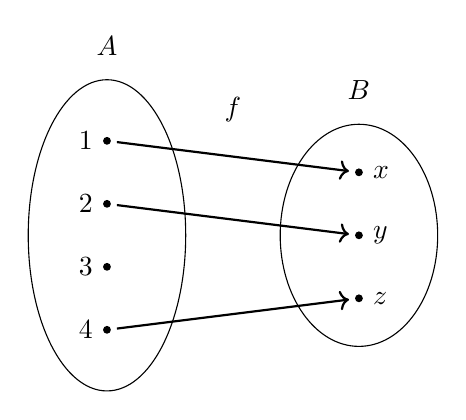
\begin{tikzpicture}[scale=0.8, ele/.style={fill=black,circle,minimum width=.8pt,inner sep=1pt},every fit/.style={ellipse,draw,inner sep=4pt}]
      \node[ele,label=left:$1$] (a1) at (0,4) {};
      \node[ele,label=left:$2$] (a2) at (0,3) {};
      \node[ele,label=left:$3$] (a3) at (0,2) {};
      \node[ele,label=left:$4$] (a4) at (0,1) {};

      \node[ele,,label=right:$z$] (b3) at (4,1.5) {};
      \node[ele,,label=right:$y$] (b2) at (4,2.5) {};
      \node[ele,,label=right:$x$] (b1) at (4,3.5) {};

      \node[draw,fit= (a1) (a2) (a3) (a4),minimum width=2cm] {} ;
      \node[draw,fit= (b1) (b2) (b3),minimum width=2cm] {} ;
      \draw[->,thick,shorten <=2pt,shorten >=2] (a1) -- (b1);
      \draw[->,thick,shorten <=2pt,shorten >=2] (a2) -- (b2);
      \draw[->,thick,shorten <=2pt,shorten >=2] (a4) -- (b3);
      \node at (2,4.5) {$f$};
      \node at (0,5.5) {$A$};
      \node at (4,4.8) {$B$};
    \end{tikzpicture}
  \end{center}
\end{multicols}

Let $f:A \to B$ is a mapping, $a$ is an element in $A$. If $a$ is mapped to $b$
under the mapping $f$, then $b$ is said to be the image of $a$ under the
mapping $f$, denoted as $b = f(a)$; $a$ is said to be the preimage of $b$ under
the mapping $f$. In the diagram above, under the mapping $f$, the image of $1$,
$2$, and $4$ are $x$, $y$, and $z$ respectively, while the preimage of $x$,
$y$, and $z$ are $1$, $2$, and $4$ respectively.

\begin{mdframed}[style=MyFrame]
  Let $A$ and $B$ be two non-empty sets, $f$ is a mapping from $A$ to $B$ such that for all elements in $A$, there is a unique corresponding element in $B$, then $f$ is a function or a mapping from $A$ to $B$, denoted as $f:A \to B$.
\end{mdframed}

The mapping shown in the diagram below is a function.
\begin{center}
  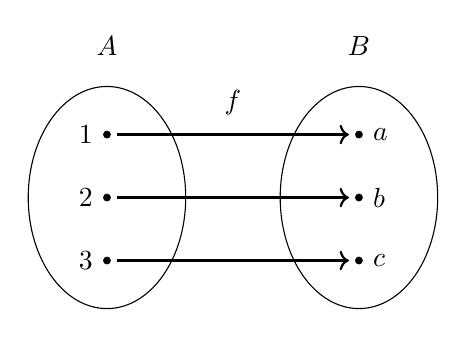
\begin{tikzpicture}[scale=0.8, ele/.style={fill=black,circle,minimum width=.8pt,inner sep=1pt},every fit/.style={ellipse,draw,inner sep=4pt}]
    \node[ele,label=left:$1$] (a1) at (0,4) {};
    \node[ele,label=left:$2$] (a2) at (0,3) {};
    \node[ele,label=left:$3$] (a3) at (0,2) {};

    \node[ele,,label=right:$c$] (b3) at (4,2) {};
    \node[ele,,label=right:$b$] (b2) at (4,3) {};
    \node[ele,,label=right:$a$] (b1) at (4,4) {};

    \node[draw,fit= (a1) (a2) (a3),minimum width=2cm] {} ;
    \node[draw,fit= (b1) (b2) (b3),minimum width=2cm] {} ;
    \draw[->,thick,shorten <=2pt,shorten >=2] (a1) -- (b1);
    \draw[->,thick,shorten <=2pt,shorten >=2] (a2) -- (b2);
    \draw[->,thick,shorten <=2pt,shorten >=2] (a3) -- (b3);
    \node at (2,4.5) {$f$};
    \node at (0,5.4) {$A$};
    \node at (4,5.4) {$B$};
  \end{tikzpicture}
\end{center}

\subsection*{Practice 1}

\setlength{\columnseprule}{1pt}
\setlength{\columnsep}{24pt}

\begin{multicols}{2}

  \begin{enumerate}
    \item For the following mappings, list the image of each element in $A$ and the
          preimage of each element in $B$, and determine whether the mapping is a
          function or not:
          \begin{enumerate}[]
            \item \adjustbox{valign=t}{
                    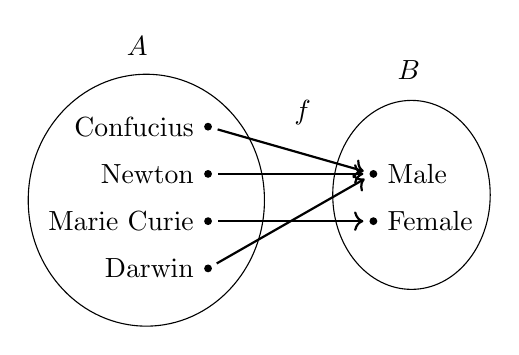
\begin{tikzpicture}[scale=0.6, ele/.style={fill=black,circle,minimum width=.8pt,inner sep=1pt},every fit/.style={ellipse,draw,inner sep=4pt}]
                      \node[ele,label=left:Confucius] (a1) at (0.5,4) {};
                      \node[ele,label=left:Newton] (a2) at (0.5,3) {};
                      \node[ele,label=left:Marie Curie] (a3) at (0.5,2) {};
                      \node[ele,label=left:Darwin] (a4) at (0.5,1) {};
                      \node[label=left:] (a999) at (-2,1) {};

                      \node[ele,,label=right:Female] (b2) at (4,2) {};
                      \node[ele,,label=right:Male] (b1) at (4,3) {};
                      \node[] (b999) at (5.5,3) {};

                      \node[draw,fit= (a1) (a2) (a3) (a4) (a999),minimum width=3cm] {} ;
                      \node[draw,fit= (b1) (b2) (b999),minimum width=2cm, minimum height=2.4cm] {} ;
                      \draw[->,thick,shorten <=2pt,shorten >=2] (a1) -- (b1);
                      \draw[->,thick,shorten <=2pt,shorten >=2] (a2) -- (b1);
                      \draw[->,thick,shorten <=2pt,shorten >=2] (a3) -- (b2);
                      \draw[->,thick,shorten <=2pt,shorten >=2] (a4) -- (b1);
                      \node at (2.5,4.3) {$f$};
                      \node at (-1,5.7) {$A$};
                      \node at (4.75,5.2) {$B$};
                    \end{tikzpicture}
                  }

            \item \adjustbox{valign=t}{
                    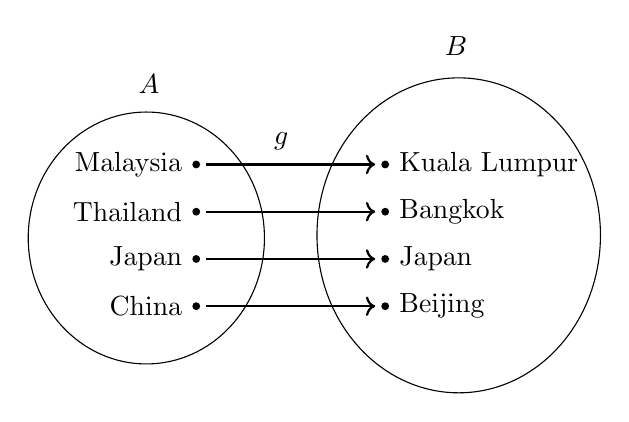
\begin{tikzpicture}[scale=0.6, ele/.style={fill=black,circle,minimum width=.8pt,inner sep=1pt},every fit/.style={ellipse,draw,inner sep=4pt}]
                      \node[ele,label=left:Malaysia] (a1) at (0,4) {};
                      \node[ele,label=left:Thailand] (a2) at (0,3) {};
                      \node[ele,label=left:Japan] (a3) at (0,2) {};
                      \node[ele,label=left:China] (a4) at (0,1) {};
                      \node[label=left:] (a999) at (-2,1) {};

                      \node[ele,,label=right:Kuala Lumpur] (b1) at (4,4) {};
                      \node[ele,,label=right:Bangkok] (b2) at (4,3) {};
                      \node[ele,,label=right:Japan] (b3) at (4,2) {};
                      \node[ele,,label=right:Beijing] (b4) at (4,1) {};
                      \node[] (b999) at (7,3) {};

                      \node[draw,fit= (a1) (a2) (a3) (a4) (a999),minimum width=3cm] {} ;
                      \node[draw,fit= (b1) (b2) (b3) (b4) (b999),minimum width=3.6cm, minimum height=4cm] {} ;
                      \draw[->,thick,shorten <=2pt,shorten >=2] (a1) -- (b1);
                      \draw[->,thick,shorten <=2pt,shorten >=2] (a2) -- (b2);
                      \draw[->,thick,shorten <=2pt,shorten >=2] (a3) -- (b3);
                      \draw[->,thick,shorten <=2pt,shorten >=2] (a4) -- (b4);
                      \node at (1.8,4.5) {$g$};
                      \node at (-1,5.7) {$A$};
                      \node at (5.5,6.5) {$B$};
                    \end{tikzpicture}
                  }

            \item \adjustbox{valign=t}{
                    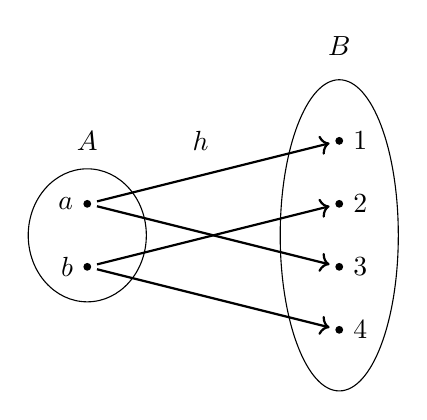
\begin{tikzpicture}[scale=0.8, ele/.style={fill=black,circle,minimum width=.8pt,inner sep=1pt},every fit/.style={ellipse,draw,inner sep=4pt}]
                      \node[ele,label=left:$a$] (a1) at (0,3) {};
                      \node[ele,label=left:$b$] (a2) at (0,2) {};

                      \node[ele,,label=right:$1$] (b1) at (4,4) {};
                      \node[ele,,label=right:$2$] (b2) at (4,3) {};
                      \node[ele,,label=right:$3$] (b3) at (4,2) {};
                      \node[ele,,label=right:$4$] (b4) at (4,1) {};

                      \node[draw,fit= (a1) (a2),minimum width=1.5cm] {} ;
                      \node[draw,fit= (b1) (b2) (b3) (b4),minimum width=1.5cm] {} ;
                      \draw[->,thick,shorten <=2pt,shorten >=2] (a1) -- (b1);
                      \draw[->,thick,shorten <=2pt,shorten >=2] (a2) -- (b2);
                      \draw[->,thick,shorten <=2pt,shorten >=2] (a1) -- (b3);
                      \draw[->,thick,shorten <=2pt,shorten >=2] (a2) -- (b4);
                      \node at (1.8,4) {$h$};
                      \node at (0,4) {$A$};
                      \node at (4,5.5) {$B$};
                    \end{tikzpicture}
                  }

            \item \adjustbox{valign=t}{
                    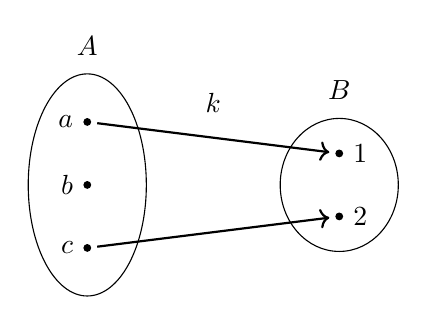
\begin{tikzpicture}[scale=0.8, ele/.style={fill=black,circle,minimum width=.8pt,inner sep=1pt},every fit/.style={ellipse,draw,inner sep=4pt}]
                      \node[ele,label=left:$a$] (a1) at (0,3) {};
                      \node[ele,label=left:$b$] (a2) at (0,2) {};
                      \node[ele,label=left:$c$] (a3) at (0,1) {};

                      \node[ele,,label=right:$1$] (b1) at (4,2.5) {};
                      \node[ele,,label=right:$2$] (b2) at (4,1.5) {};

                      \node[draw,fit= (a1) (a2) (a3),minimum width=1.5cm] {} ;
                      \node[draw,fit= (b1) (b2),minimum width=1.5cm] {} ;
                      \draw[->,thick,shorten <=2pt,shorten >=2] (a1) -- (b1);
                      \draw[->,thick,shorten <=2pt,shorten >=2] (a3) -- (b2);
                      \node at (2,3.3) {$k$};
                      \node at (0,4.2) {$A$};
                      \node at (4,3.5) {$B$};
                    \end{tikzpicture}
                  }
          \end{enumerate}

    \item Given a mapping $g:x \to x+3$, $x \in\big\{$-2, -1, 0, 1, 2, 3$\big\}$, find
          the image of each $x$.

    \item Determine whether the following mappings are functions.
          \begin{enumerate}
            \item \adjustbox{valign=t}{
                    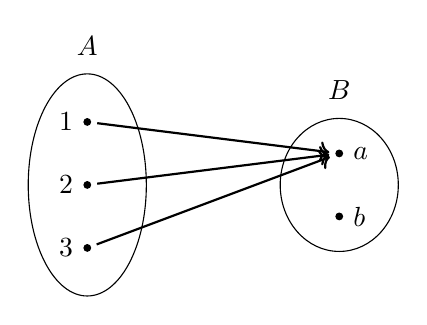
\begin{tikzpicture}[scale=0.8, ele/.style={fill=black,circle,minimum width=.8pt,inner sep=1pt},every fit/.style={ellipse,draw,inner sep=4pt}]
                      \node[ele,label=left:$1$] (a1) at (0,3) {};
                      \node[ele,label=left:$2$] (a2) at (0,2) {};
                      \node[ele,label=left:$3$] (a3) at (0,1) {};

                      \node[ele,,label=right:$a$] (b1) at (4,2.5) {};
                      \node[ele,,label=right:$b$] (b2) at (4,1.5) {};

                      \node[draw,fit= (a1) (a2) (a3),minimum width=1.5cm] {} ;
                      \node[draw,fit= (b1) (b2),minimum width=1.5cm] {} ;
                      \draw[->,thick,shorten <=2pt,shorten >=2] (a1) -- (b1);
                      \draw[->,thick,shorten <=2pt,shorten >=2] (a2) -- (b1);
                      \draw[->,thick,shorten <=2pt,shorten >=2] (a3) -- (b1);
                      \node at (0,4.2) {$A$};
                      \node at (4,3.5) {$B$};
                    \end{tikzpicture}
                  }

            \item \adjustbox{valign=t}{
                    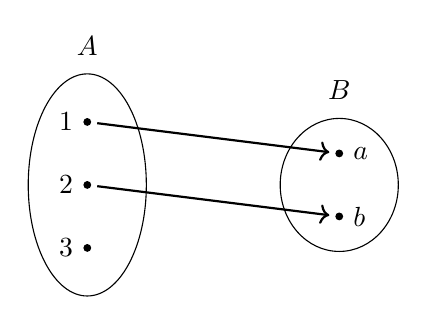
\begin{tikzpicture}[scale=0.8, ele/.style={fill=black,circle,minimum width=.8pt,inner sep=1pt},every fit/.style={ellipse,draw,inner sep=4pt}]
                      \node[ele,label=left:$1$] (a1) at (0,3) {};
                      \node[ele,label=left:$2$] (a2) at (0,2) {};
                      \node[ele,label=left:$3$] (a3) at (0,1) {};

                      \node[ele,,label=right:$a$] (b1) at (4,2.5) {};
                      \node[ele,,label=right:$b$] (b2) at (4,1.5) {};

                      \node[draw,fit= (a1) (a2) (a3),minimum width=1.5cm] {} ;
                      \node[draw,fit= (b1) (b2),minimum width=1.5cm] {} ;
                      \draw[->,thick,shorten <=2pt,shorten >=2] (a1) -- (b1);
                      \draw[->,thick,shorten <=2pt,shorten >=2] (a2) -- (b2);
                      \node at (0,4.2) {$A$};
                      \node at (4,3.5) {$B$};
                    \end{tikzpicture}
                  }

            \item \adjustbox{valign=t}{
                    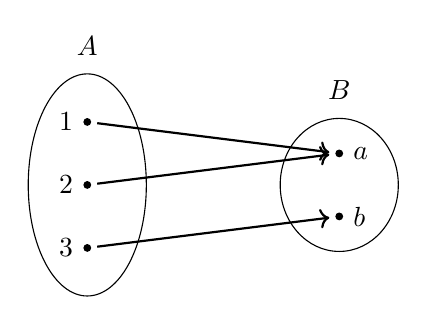
\begin{tikzpicture}[scale=0.8, ele/.style={fill=black,circle,minimum width=.8pt,inner sep=1pt},every fit/.style={ellipse,draw,inner sep=4pt}]
                      \node[ele,label=left:$1$] (a1) at (0,3) {};
                      \node[ele,label=left:$2$] (a2) at (0,2) {};
                      \node[ele,label=left:$3$] (a3) at (0,1) {};

                      \node[ele,,label=right:$a$] (b1) at (4,2.5) {};
                      \node[ele,,label=right:$b$] (b2) at (4,1.5) {};

                      \node[draw,fit= (a1) (a2) (a3),minimum width=1.5cm] {} ;
                      \node[draw,fit= (b1) (b2),minimum width=1.5cm] {} ;
                      \draw[->,thick,shorten <=2pt,shorten >=2] (a1) -- (b1);
                      \draw[->,thick,shorten <=2pt,shorten >=2] (a2) -- (b1);
                      \draw[->,thick,shorten <=2pt,shorten >=2] (a3) -- (b2);
                      \node at (0,4.2) {$A$};
                      \node at (4,3.5) {$B$};
                    \end{tikzpicture}
                  }

            \item \adjustbox{valign=t}{
                    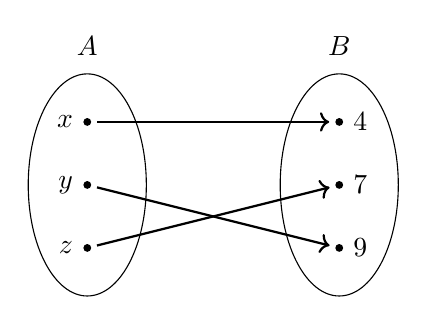
\begin{tikzpicture}[scale=0.8, ele/.style={fill=black,circle,minimum width=.8pt,inner sep=1pt},every fit/.style={ellipse,draw,inner sep=4pt}]
                      \node[ele,label=left:$x$] (a1) at (0,3) {};
                      \node[ele,label=left:$y$] (a2) at (0,2) {};
                      \node[ele,label=left:$z$] (a3) at (0,1) {};

                      \node[ele,,label=right:$4$] (b1) at (4,3) {};
                      \node[ele,,label=right:$7$] (b2) at (4,2) {};
                      \node[ele,,label=right:$9$] (b3) at (4,1) {};

                      \node[draw,fit= (a1) (a2) (a3),minimum width=1.5cm] {} ;
                      \node[draw,fit= (b1) (b2) (b3),minimum width=1.5cm] {} ;
                      \draw[->,thick,shorten <=2pt,shorten >=2] (a1) -- (b1);
                      \draw[->,thick,shorten <=2pt,shorten >=2] (a2) -- (b3);
                      \draw[->,thick,shorten <=2pt,shorten >=2] (a3) -- (b2);
                      \node at (0,4.2) {$A$};
                      \node at (4,4.2) {$B$};
                    \end{tikzpicture}
                  }

            \item \adjustbox{valign=t}{
                    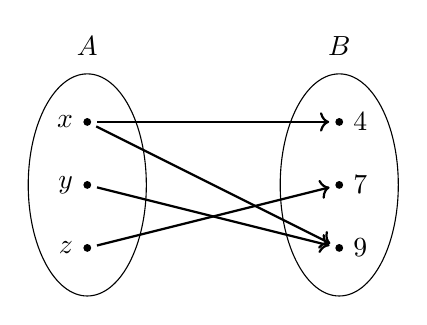
\begin{tikzpicture}[scale=0.8, ele/.style={fill=black,circle,minimum width=.8pt,inner sep=1pt},every fit/.style={ellipse,draw,inner sep=4pt}]
                      \node[ele,label=left:$x$] (a1) at (0,3) {};
                      \node[ele,label=left:$y$] (a2) at (0,2) {};
                      \node[ele,label=left:$z$] (a3) at (0,1) {};

                      \node[ele,,label=right:$4$] (b1) at (4,3) {};
                      \node[ele,,label=right:$7$] (b2) at (4,2) {};
                      \node[ele,,label=right:$9$] (b3) at (4,1) {};

                      \node[draw,fit= (a1) (a2) (a3),minimum width=1.5cm] {} ;
                      \node[draw,fit= (b1) (b2) (b3),minimum width=1.5cm] {} ;
                      \draw[->,thick,shorten <=2pt,shorten >=2] (a1) -- (b1);
                      \draw[->,thick,shorten <=2pt,shorten >=2] (a1) -- (b3);
                      \draw[->,thick,shorten <=2pt,shorten >=2] (a2) -- (b3);
                      \draw[->,thick,shorten <=2pt,shorten >=2] (a3) -- (b2);
                      \node at (0,4.2) {$A$};
                      \node at (4,4.2) {$B$};
                    \end{tikzpicture}
                  }

            \item \adjustbox{valign=t}{
                    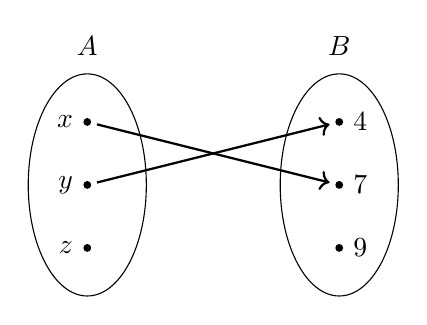
\begin{tikzpicture}[scale=0.8, ele/.style={fill=black,circle,minimum width=.8pt,inner sep=1pt},every fit/.style={ellipse,draw,inner sep=4pt}]
                      \node[ele,label=left:$x$] (a1) at (0,3) {};
                      \node[ele,label=left:$y$] (a2) at (0,2) {};
                      \node[ele,label=left:$z$] (a3) at (0,1) {};

                      \node[ele,,label=right:$4$] (b1) at (4,3) {};
                      \node[ele,,label=right:$7$] (b2) at (4,2) {};
                      \node[ele,,label=right:$9$] (b3) at (4,1) {};

                      \node[draw,fit= (a1) (a2) (a3),minimum width=1.5cm] {} ;
                      \node[draw,fit= (b1) (b2) (b3),minimum width=1.5cm] {} ;
                      \draw[->,thick,shorten <=2pt,shorten >=2] (a1) -- (b2);
                      \draw[->,thick,shorten <=2pt,shorten >=2] (a2) -- (b1);
                      \node at (0,4.2) {$A$};
                      \node at (4,4.2) {$B$};
                    \end{tikzpicture}
                  }
          \end{enumerate}
  \end{enumerate}

\end{multicols}

The function $f: A \to B$ can be written as $y = f(x)$, $x$ is the element of
$A$ and $y$ is the element of $B$. When $x$ changes, $y$ changes as well. $x$
is called independent variable, while $y$ is called dependent variable.

Keep in mind that $f(x)$ is NOT the product of $f$ and $x$.

\subsection*{Representation of Functions}

Generally speaking, there are a few ways to represent a function:
\begin{enumerate}
  \item \textbf{Narrative Form}: express the function of two sets in words. For example, Let $A = \big\{1, 2, 3\big\}$ and $B = \big\{1, 4, 9\big\}$, $f$ is a function from $A$ to $B$, its definition is that for any element $x$ in $A$, its corresponding element is $x^2$ in $B$.
  \item \textbf{Arrow Method}: draw an arrow to connect the preimage and image of a function such that the preimage is corresponding to the image. To express the example above, we express it as $f: 1 \to 1,\ 2 \to 4,\ 3 \to 9$.
  \item \textbf{Analytical Method}: express the function in the form of mathematical expression to represent the relationship between the independent variable and the dependent variable. For example, $f(x) = x^2, x \in A$.
  \item \textbf{Venn Diagram}: draw arrows between the venn diagram of two sets to represent the function, as shown below:
        \begin{center}
          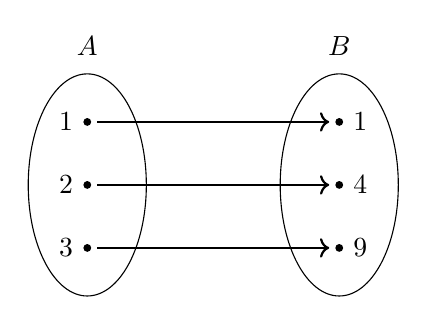
\begin{tikzpicture}[scale=0.8, ele/.style={fill=black,circle,minimum width=.8pt,inner sep=1pt},every fit/.style={ellipse,draw,inner sep=4pt}]
            \node[ele,label=left:$1$] (a1) at (0,3) {};
            \node[ele,label=left:$2$] (a2) at (0,2) {};
            \node[ele,label=left:$3$] (a3) at (0,1) {};

            \node[ele,,label=right:$1$] (b1) at (4,3) {};
            \node[ele,,label=right:$4$] (b2) at (4,2) {};
            \node[ele,,label=right:$9$] (b3) at (4,1) {};

            \node[draw,fit= (a1) (a2) (a3),minimum width=1.5cm] {} ;
            \node[draw,fit= (b1) (b2) (b3),minimum width=1.5cm] {} ;
            \draw[->,thick,shorten <=2pt,shorten >=2] (a1) -- (b1);
            \draw[->,thick,shorten <=2pt,shorten >=2] (a2) -- (b2);
            \draw[->,thick,shorten <=2pt,shorten >=2] (a3) -- (b3);
            \node at (0,4.2) {$A$};
            \node at (4,4.2) {$B$};
          \end{tikzpicture}
        \end{center}
  \item \textbf{Table Method}: express the function in the form of table, showing the relationship of the chosen value between independent variable $x$ and the value of its corresponding dependent variable $y$, as shown below:
        \begin{center}
          \begin{tabular}{|c|c|c|c|}
            \hline
            $x$ & $1$ & $2$ & $3$ \\
            \hline
            $y$ & $1$ & $4$ & $9$ \\
            \hline
          \end{tabular}
        \end{center}

  \item \textbf{Graphical Method}: draw a graph to represent the function of the two variables, as shown below:
        \begin{center}
          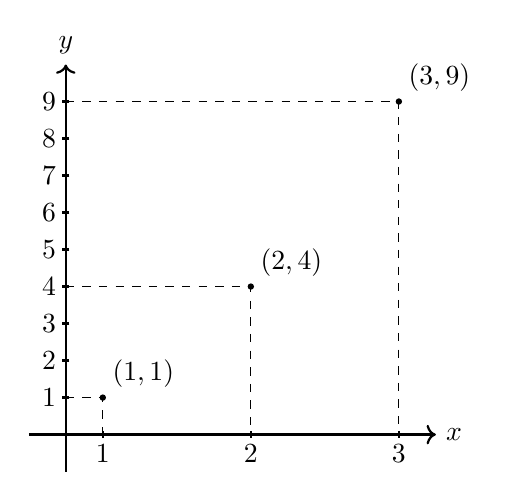
\begin{tikzpicture}[scale=0.47]
            \draw[->,thick] (-1,0) -- (10,0) node[right] {$x$};
            \draw[->,thick] (0,-1) -- (0,10) node[above] {$y$};
            \draw[thick] (1,0.1) -- (1,-0.1);
            \node[below] at (1,0) {1};
            \draw[thick] (5,0.1) -- (5,-0.1);
            \node[below] at (5,0) {2};
            \draw[thick] (9,0.1) -- (9,-0.1);
            \node[below] at (9,0) {3};
            \foreach \y in {1,...,9}
              {
                \draw[thick] (0.1,\y) -- (-0.1,\y);
                \node[left] at (0,\y) {\y};
              }
            \filldraw (1, 1) circle (2pt) node[above right]{$(1,1)$};
            \filldraw (5, 4) circle (2pt) node[above right]{$(2,4)$};
            \filldraw (9, 9) circle (2pt) node[above right]{$(3,9)$};
            \draw[dashed] (0,1) -- (1,1) -- (1,0);
            \draw[dashed] (0,4) -- (5,4) -- (5,0);
            \draw[dashed] (0,9) -- (9,9) -- (9,0);
          \end{tikzpicture}
        \end{center}
\end{enumerate}

\subsection*{Practice 2}

\setlength{\columnseprule}{1pt}
\setlength{\columnsep}{24pt}

\begin{multicols}{2}

  Express the following functions using analytical method, venn diagram, table
  method and graphical method.
  \begin{enumerate}[label=(\alph*)]
    \item $f$ mapping each integers from $-3$ to $3$ to its squares plus $4$.
    \item $g$ mapping each natural numbers from $1$ to $4$ to its cubes.
  \end{enumerate}

\end{multicols}

\subsection*{Exercise 22.1}

\setlength{\columnseprule}{1pt}
\setlength{\columnsep}{24pt}

\begin{multicols}{2}

  \begin{enumerate}
    \item Express the mapping from set $A$ to set $B$, and determine which of the
          following mappings are functions.

          \resizebox{22em}{!}{
            \begin{tabular}{|c|c|c|c|}
              \hline
                  & Set $A$                                & Set $B$                                                                   & Mapping       \\
              \hline
              (a) & \{0, 3, 9, 12\}                        & \{0, 1, 2, 3\}                                                            & Divide by $3$ \\
              \hline
              (b) & \{-2, -1, 0, 1, 2\}                    & \{0, 1, 4, 9, 16\}                                                        & Power of $4$  \\
              \hline
              (c) & \{-2, -1, 0, 1, 2\}                    & \{0, 1, 4\}                                                               & Square        \\
              \hline
              (d) & \{30$^\circ$, 45$^\circ$, 60$^\circ$\} & $\left\{\dfrac{1}{2},\ \dfrac{\sqrt{2}}{2},\ \dfrac{\sqrt{3}}{2}\right\}$ & Sine          \\
              \hline
              (e) & \{-1, 0, 1, 2\}                        & \{-1, 0, 1\}                                                              & Cube          \\
              \hline
            \end{tabular}
          }

    \item Let function $f(x) = 3x^2 + 1$.
          \begin{enumerate}
            \item Find the image of the following elements:
                  \begin{enumerate}
                    \item -3
                    \item -2
                    \item 0
                    \item 2
                    \item 5
                  \end{enumerate}
            \item Find the preimage of the following elements:
                  \begin{enumerate}
                    \item 13
                    \item 28
                    \item 1
                    \item 0
                    \item 4
                  \end{enumerate}
          \end{enumerate}

    \item Let function $g(x) = 5x-2$. Find:
          \begin{enumerate}
            \item $g(-2)$
            \item $g(-1)$
            \item $g(0)$
          \end{enumerate}

    \item Let function $f(x) = \left\{\begin{array}{ll}
              \ \ \ \ \ \ 2x, & x \leq -1     \\
              \ \ x-1,        & -1 \leq x < 3 \\
              4x + 2,         & x \geq 3
            \end{array}\right.$, find

          \begin{enumerate}
            \item $f(-5)$
            \item $f(-2)$
            \item $f(0)$
            \item $f(2)$
            \item $f(10)$
          \end{enumerate}

    \item Let $f: \mathbb{R} \to \mathbb{R}$, $f(x) = x^4$. Find the image of $-1$, 0, 1,
          and 2 under $f$.

    \item Let $f: \mathbb{R} \to \mathbb{R}$, $f(x) = x^4$. Find the preimage of 0, 1,
          and 4 under $f$.

          In $\mathbb{R}$, which element does not have a preimage?

    \item In the diagram below, given that function $g: A \to B$ is defined as $g: x \to
            2x - 8$. Find the value of $a$ and $b$.
          \begin{center}
            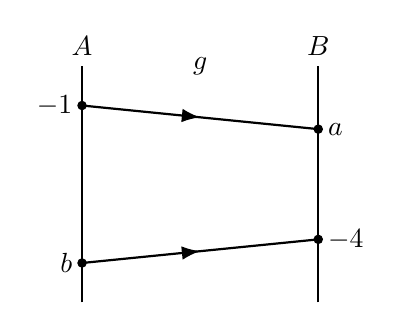
\begin{tikzpicture}
              \draw[thick] (0,0) -- (0,3) node[above]{$A$};
              \draw[thick] (3,0) -- (3,3) node[above]{$B$};
              \node at (1.5, 3) {$g$};
              \filldraw (0, 2.5) circle (1.5pt) node[left]{$-1$};
              \filldraw (0, 0.5) circle (1.5pt) node[left]{$b$};
              \filldraw (3, 0.8) circle (1.5pt) node[right]{$-4$};
              \filldraw (3, 2.2) circle (1.5pt) node[right]{$a$};
              \begin{scope}[thick,decoration={
                      markings,
                      mark=at position 0.5 with {\arrow{Latex}}}
                ]
                \draw[postaction={decorate}] (0, 2.5) -- (3, 2.2);
                \draw[postaction={decorate}] (0, 0.5) -- (3, 0.8);
              \end{scope}
            \end{tikzpicture}
          \end{center}

    \item Using narrative form, arrow method, venn diagram, table method and graphical
          method, express the function $f(x) = 2x$, $x \in \{-2, -1, 0, 1, 2\}$.
  \end{enumerate}
\end{multicols}
\newpage
\section{Domain and Range}

\begin{mdframed}[style=MyFrame]
  Let $f$ is a function from set $A$ to set $B$, then set $A$ is called the domain of $f$, denoted by $D_f$; set $B$ is called the codomain of $f$; the set of the images of all elements of $A$ under $f$ is called the range of $f$, denoted by $R_f$.
\end{mdframed}

If the domain $A$ and range $B$ of function $f: A\to B$ are both subsets of
real number set $\mathbb{R}$, then this function is called real valued function
/ real function. This book primarily discusses about real valued functions.
When the domain of a real function is not mentioned and only the mapping rule
is given, its domain is assumed to be the set of all real numbers that yield
defined values $f(x)$. After the domain and the mapping rule are determined,
the range of a function will then be determined.

\begin{center}
  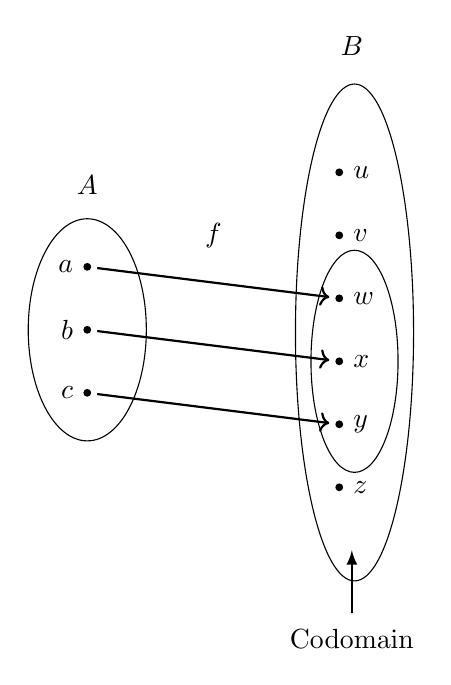
\begin{tikzpicture}[scale=0.8, ele/.style={fill=black,circle,minimum width=.8pt,inner sep=1pt},every fit/.style={ellipse,draw,inner sep=4pt}]
    \node[ele,label=left:$a$] (a1) at (0,4.5) {};
    \node[ele,label=left:$b$] (a2) at (0,3.5) {};
    \node[ele,label=left:$c$] (a3) at (0,2.5) {};

    \node[ele,,label=right:$u$] (b1) at (4,6) {};
    \node[ele,,label=right:$v$] (b2) at (4,5) {};
    \node[ele,,label=right:$w$] (b3) at (4,4) {};
    \node[ele,,label=right:$x$] (b4) at (4,3) {};
    \node[ele,,label=right:$y$] (b5) at (4,2) {};
    \node[ele,,label=right:$z$] (b6) at (4,1) {};
    \node[] (b999) at (4.4,1) {};
    \node[] (b998) at (4.4,3) {};

    \node[draw,fit= (a1) (a2) (a3),minimum width=1.5cm] {} ;
    \node[draw,fit= (b1) (b2) (b3) (b4) (b5) (b6) (b999),minimum width=1.5cm] {} ;
    \node[draw,fit= (b3) (b4) (b5) (b998),minimum width=1cm] {} ;
    \draw[->,thick,shorten <=2pt,shorten >=2] (a1) -- (b3);
    \draw[->,thick,shorten <=2pt,shorten >=2] (a2) -- (b4);
    \draw[->,thick,shorten <=2pt,shorten >=2] (a3) -- (b5);
    \node at (0,5.8) {$A$};
    \node at (4.2,8) {$B$};
    \node at (2,5) {$f$};
    \draw[thick, -latex](4.2,-1) -- (4.2,0);
    \node at (4.2,-1.4) {Codomain};
  \end{tikzpicture}
\end{center}

\begin{mdframed}[style=MyFrame]
  \large{\textbf{Interval Notation}}
  \normalsize

  \noindent Let $a$ and $b$ be two real number, $a < b$.
  \begin{center}
    \begin{tabular}{|c|c|}
      \hline
      Intervals      & Set Notations                                          \\
      \hline
      $(a, b)$       & $\left\{x | x \in \mathbb{R}, a < x < b\right\}$       \\
      $[a, b)$       & $\left\{x | x \in \mathbb{R}, a \leq x < b\right\}$    \\
      $(a, b]$       & $\left\{x | x \in \mathbb{R}, a < x \leq b\right\}$    \\
      $[a, b]$       & $\left\{x | x \in \mathbb{R}, a \leq x \leq b\right\}$ \\
      $(a, \infty)$  & $\left\{x | x \in \mathbb{R}, x > a\right\}$           \\
      $[a, \infty)$  & $\left\{x | x \in \mathbb{R}, x \leq a\right\}$        \\
      $(-\infty, a)$ & $\left\{x | x \in \mathbb{R}, x < a\right\}$           \\
      $(-\infty, a]$ & $\left\{x | x \in \mathbb{R}, x \leq a\right\}$        \\
      \hline
    \end{tabular}
  \end{center}
\end{mdframed}

\subsection*{Practice 3}

\setlength{\columnseprule}{1pt}
\setlength{\columnsep}{24pt}

\begin{multicols}{2}

  \begin{enumerate}
    \item Let $A = \{2, 4, 5, 7\}$ and $B = \{3, 5, 7, 8, 9\}$, the definition of
          function $g$ is given by the diagram below. Find the domain, codomain and range
          of function $g$.
          \begin{center}
            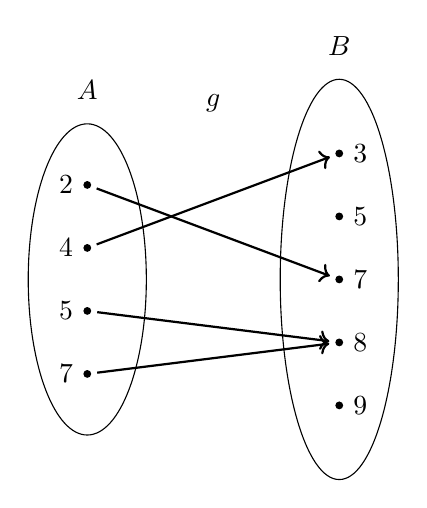
\begin{tikzpicture}[scale=0.8, ele/.style={fill=black,circle,minimum width=.8pt,inner sep=1pt},every fit/.style={ellipse,draw,inner sep=4pt}]
              \node[ele,label=left:$2$] (a1) at (0,3.5) {};
              \node[ele,label=left:$4$] (a2) at (0,2.5) {};
              \node[ele,label=left:$5$] (a3) at (0,1.5) {};
              \node[ele,label=left:$7$] (a4) at (0,0.5) {};

              \node[ele,,label=right:$3$] (b1) at (4,4) {};
              \node[ele,,label=right:$5$] (b2) at (4,3) {};
              \node[ele,,label=right:$7$] (b3) at (4,2) {};
              \node[ele,,label=right:$8$] (b4) at (4,1) {};
              \node[ele,,label=right:$9$] (b5) at (4,0) {};

              \node[draw,fit= (a1) (a2) (a3) (a4),minimum width=1.5cm] {} ;
              \node[draw,fit= (b1) (b2) (b3) (b4) (b5),minimum width=1.5cm] {} ;
              \draw[->,thick,shorten <=2pt,shorten >=2] (a1) -- (b3);
              \draw[->,thick,shorten <=2pt,shorten >=2] (a2) -- (b1);
              \draw[->,thick,shorten <=2pt,shorten >=2] (a3) -- (b4);
              \draw[->,thick,shorten <=2pt,shorten >=2] (a4) -- (b4);
              \node at (0,5) {$A$};
              \node at (4,5.7) {$B$};
              \node at (2,4.8) {$g$};
            \end{tikzpicture}
          \end{center}

    \item Let $A = \{-2, -1, 0, 1, 2\}$, function $f: A \to \mathbb{R}$ is defined by
          $f(x) = x^2 - 1$. Find the domain and range of $f$.

    \item The curve in the diagram below represents the function $y = f(x)$, $-2 \leq x
            \leq 3$. Find the domain and range of $f$.
          \begin{center}
            \begin{tikzpicture}
              \begin{axis}[
                  axis lines=middle,
                  xmin=-2.5, xmax=3.5,
                  ymin=-3, ymax=8,
                  xtick={-2,-1,0,1,2,3},
                  ytick={-2, -1, ..., 7},
                  xlabel={$x$},
                  ylabel={$y$},
                  xlabel style={anchor=east, xshift=0.5cm},
                  ylabel style={anchor=north, yshift=0.5cm},
                  xtick style={thick, color=black},
                  ytick style={thick, color=black},
                  line style={thick, color=black},
                ]
                \addplot[domain=-2:3, thick] {x^2 - 2};
                \path (axis cs:0,0)
                node [anchor=north east, xshift=0.05cm] {0};
                \draw[dashed] (axis cs:0,7) -- (axis cs:3,7);
                \filldraw (axis cs:3,7) circle (1.6pt);
                \draw[dashed] (axis cs:0,2) -- (axis cs:-2,2);
                \filldraw (axis cs:-2,2) circle (1.6pt);
              \end{axis}
            \end{tikzpicture}
          \end{center}

    \item Find the domain and range of the following functions:
          \begin{enumerate}
            \item $f(x) = -4x + 5$
            \item $g(x) = x^2 - 1$
            \item $h(x) = \dfrac{1}{4x + 7}$
            \item $k(x) = \sqrt{6 - x}$
          \end{enumerate}
  \end{enumerate}

\end{multicols}

\subsection*{Exercise 22.2}

\setlength{\columnseprule}{1pt}
\setlength{\columnsep}{24pt}

\begin{multicols}{2}

  \begin{enumerate}
    \item Let $X = \{a, b, c, d\}$ and $Y = \{-1, 2, 9, 11\}$, function $f: X \to Y$ is
          defined by $f(a) = 2$, $f(b) = -1$, $f(c) = 2$, $f(d) = 9$. Find the domain and
          range of the $f$.

    \item The curve in the diagram below represents the function $y = f(x)$, $-1 < x \leq
            4$. Find the domain and range of $f$.
          \begin{center}
            \begin{tikzpicture}
              \begin{axis}[
                  axis lines=middle,
                  xmin=-2.5, xmax=4.5,
                  ymin=-4, ymax=8,
                  xtick={-2,-1,0,1,2,3,4},
                  ytick={-3, -2, -1, ..., 7},
                  xlabel={$x$},
                  ylabel={$y$},
                  xlabel style={anchor=east, xshift=0.5cm},
                  ylabel style={anchor=north, yshift=0.5cm},
                  xtick style={thick, color=black},
                  ytick style={thick, color=black},
                  line style={thick, color=black},
                ]
                \addplot[domain=-1:4, thick] {-(x - 1)^2 + 6};
                \path (axis cs:0,0)
                node [anchor=north east, xshift=0.05cm] {0};
                \draw[dashed] (axis cs:0,-3) -- (axis cs:4,-3);
                \filldraw (axis cs:4,-3) circle (1.6pt);
                \draw[dashed] (axis cs:0,2) -- (axis cs:-1,2);
                \filldraw[fill=white] (axis cs:-1,2) circle (1.6pt);
              \end{axis}
            \end{tikzpicture}
          \end{center}

    \item Let $A = \{a, b, c, d, e\}$ and $B = \{4, 5, 8, 9, 12\}$, the definition of
          function $g: A \to B$ is given by the digram below. Find the domain, codomain
          and range of function $g$.
          \begin{center}
            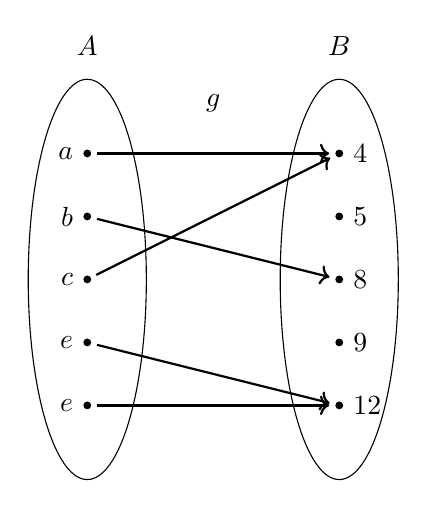
\begin{tikzpicture}[scale=0.8, ele/.style={fill=black,circle,minimum width=.8pt,inner sep=1pt},every fit/.style={ellipse,draw,inner sep=4pt}]
              \node[ele,label=left:$a$] (a1) at (0,4) {};
              \node[ele,label=left:$b$] (a2) at (0,3) {};
              \node[ele,label=left:$c$] (a3) at (0,2) {};
              \node[ele,label=left:$e$] (a4) at (0,1) {};
              \node[ele,label=left:$e$] (a5) at (0,0) {};

              \node[ele,,label=right:$4$] (b1) at (4,4) {};
              \node[ele,,label=right:$5$] (b2) at (4,3) {};
              \node[ele,,label=right:$8$] (b3) at (4,2) {};
              \node[ele,,label=right:$9$] (b4) at (4,1) {};
              \node[ele,,label=right:$12$] (b5) at (4,0) {};

              \node[draw,fit= (a1) (a2) (a3) (a4) (a5),minimum width=1.5cm] {} ;
              \node[draw,fit= (b1) (b2) (b3) (b4) (b5),minimum width=1.5cm] {} ;
              \draw[->,thick,shorten <=2pt,shorten >=2] (a1) -- (b1);
              \draw[->,thick,shorten <=2pt,shorten >=2] (a2) -- (b3);
              \draw[->,thick,shorten <=2pt,shorten >=2] (a3) -- (b1);
              \draw[->,thick,shorten <=2pt,shorten >=2] (a4) -- (b5);
              \draw[->,thick,shorten <=2pt,shorten >=2] (a5) -- (b5);
              \node at (0,5.7) {$A$};
              \node at (4,5.7) {$B$};
              \node at (2,4.8) {$g$};
            \end{tikzpicture}
          \end{center}

    \item Let $A = \{-1, 0, 1, 2\}$, function $f: A \to \mathbb{R}$ is defined by $f(x) =
            3x^2 - 2$, find the domain and range of $f$.

    \item Let $A = \{-1, 0, 2, 5, 11\}$, function $f: A \to \mathbb{R}$ is defined by
          $f(x) = x^2 - x - 2$, find the domain and range of $f$.

    \item Find the domain and range of the following functions:
          \begin{enumerate}
            \item $f(x) = x^3$
            \item $g(x) = \sqrt{1 - x^2}$
            \item $h(x) = \dfrac{1}{2x + 3}$
            \item $k(x) = x^2 - 2x + 4$
          \end{enumerate}
  \end{enumerate}

\end{multicols}

\newpage
\section{Graphs of Functions and Their Transformations}
\subsection*{Graphs of Simple Functions}

On a Cartesian plane, the graphs formed by all the point $(x, y)$ that
satisfied the equation $y = f(x)$ are called graphs of function $f$. Below are
some examples of graphs of simple functions.

Note that any line that is parallel to the $y$-axis intersects the graph of a
function at most once. \setlength{\columnseprule}{0pt}
\setlength{\columnsep}{24pt}

\begin{multicols}{2}
  \begin{enumerate}[label=(\alph*)]
    \item $y = x$
          \begin{center}
            \resizebox{0.33\textwidth}{!}{
              \begin{tikzpicture}
                \begin{axis}[
                    axis lines=middle,
                    xmin=-5.5, xmax=5.5,
                    ymin=-5.5, ymax=5.5,
                    xlabel={$x$},
                    ylabel={$y$},
                    ticks=none,
                    xlabel style={anchor=east, xshift=0.5cm},
                    ylabel style={anchor=north, yshift=0.5cm},
                    line style={thick, color=black},
                  ]
                  \addplot[domain=-5:5, thick] {x};
                  \path (axis cs:0,0)
                  node [anchor=north east, xshift=0.05cm] {$O$};
                \end{axis}
              \end{tikzpicture}
            }
          \end{center}

    \item $y = -x$
          \begin{center}
            \resizebox{0.33\textwidth}{!}{
              \begin{tikzpicture}
                \begin{axis}[
                    axis lines=middle,
                    xmin=-5.5, xmax=5.5,
                    ymin=-5.5, ymax=5.5,
                    xlabel={$x$},
                    ylabel={$y$},
                    ticks=none,
                    xlabel style={anchor=east, xshift=0.5cm},
                    ylabel style={anchor=north, yshift=0.5cm},
                    line style={thick, color=black},
                  ]
                  \addplot[domain=-5:5, thick] {-x};
                  \path (axis cs:0,0)
                  node [anchor=north east, xshift=0.05cm] {$O$};
                \end{axis}
              \end{tikzpicture}
            }
          \end{center}
  \end{enumerate}
\end{multicols}
\begin{multicols}{2}
  \begin{enumerate}[label=(\alph*)]
    \setcounter{enumi}{2}
    \item $y = x^2$
          \begin{center}
            \resizebox{0.33\textwidth}{!}{
              \begin{tikzpicture}
                \begin{axis}[
                    axis lines=middle,
                    xmin=-2.5, xmax=2.5,
                    ymin=-0.5, ymax=5.5,
                    xlabel={$x$},
                    ylabel={$y$},
                    ticks=none,
                    xlabel style={anchor=east, xshift=0.5cm},
                    ylabel style={anchor=north, yshift=0.5cm},
                    line style={thick, color=black},
                  ]
                  \addplot[domain=-5:5, thick] {x^2};
                  \path (axis cs:0,0)
                  node [anchor=north east, xshift=0.05cm] {$O$};
                \end{axis}
              \end{tikzpicture}
            }
          \end{center}

    \item $y = x^2$
          \begin{center}
            \resizebox{0.33\textwidth}{!}{
              \begin{tikzpicture}
                \begin{axis}[
                    axis lines=middle,
                    xmin=-2.5, xmax=2.5,
                    ymin=-5.5, ymax=0.5,
                    xlabel={$x$},
                    ylabel={$y$},
                    ticks=none,
                    xlabel style={anchor=east, xshift=0.5cm},
                    ylabel style={anchor=north, yshift=0.5cm},
                    line style={thick, color=black},
                  ]
                  \addplot[domain=-5:5, thick] {-x^2};
                  \path (axis cs:0,0)
                  node [anchor=north east, xshift=0.05cm] {$O$};
                \end{axis}
              \end{tikzpicture}
            }
          \end{center}
  \end{enumerate}
\end{multicols}
\begin{multicols}{2}
  \begin{enumerate}[label=(\alph*)]
    \setcounter{enumi}{4}
    \item $y = x^3$
          \begin{center}
            \resizebox{0.33\textwidth}{!}{
              \begin{tikzpicture}
                \begin{axis}[
                    axis lines=middle,
                    xmin=-2.5, xmax=2.5,
                    ymin=-5.5, ymax=5.5,
                    xlabel={$x$},
                    ylabel={$y$},
                    ticks=none,
                    xlabel style={anchor=east, xshift=0.5cm},
                    ylabel style={anchor=north, yshift=0.5cm},
                    line style={thick, color=black},
                  ]
                  \addplot[domain=-5:5, thick] {x^3};
                  \path (axis cs:0,0)
                  node [anchor=north east, xshift=0.05cm] {$O$};
                \end{axis}
              \end{tikzpicture}
            }
          \end{center}

    \item $y = -x^3$
          \begin{center}
            \resizebox{0.33\textwidth}{!}{
              \begin{tikzpicture}
                \begin{axis}[
                    axis lines=middle,
                    xmin=-2.5, xmax=2.5,
                    ymin=-5.5, ymax=5.5,
                    xlabel={$x$},
                    ylabel={$y$},
                    ticks=none,
                    xlabel style={anchor=east, xshift=0.5cm},
                    ylabel style={anchor=north, yshift=0.5cm},
                    line style={thick, color=black},
                  ]
                  \addplot[domain=-5:5, thick] {-x^3};
                  \path (axis cs:0,0)
                  node [anchor=north east, xshift=0.05cm] {$O$};
                \end{axis}
              \end{tikzpicture}
            }
          \end{center}
  \end{enumerate}
\end{multicols}
\newpage
\begin{multicols}{2}
  \begin{enumerate}[label=(\alph*)]
    \setcounter{enumi}{6}
    \item $y = \dfrac{1}{x}$
          \begin{center}
            \resizebox{0.33\textwidth}{!}{
              \begin{tikzpicture}
                \begin{axis}[
                    axis lines=middle,
                    xmin=-5.5, xmax=5.5,
                    ymin=-5.5, ymax=5.5,
                    xlabel={$x$},
                    ylabel={$y$},
                    ticks=none,
                    xlabel style={anchor=east, xshift=0.5cm},
                    ylabel style={anchor=north, yshift=0.5cm},
                    line style={thick, color=black},
                  ]
                  \addplot[domain=-5:-0.01, thick] {1/x};
                  \addplot[domain=0.01:5, thick] {1/x};
                  \path (axis cs:0,0)
                  node [anchor=north east, xshift=0.05cm] {$O$};
                \end{axis}
              \end{tikzpicture}
            }
          \end{center}

    \item $y = -\dfrac{1}{x}$
          \begin{center}
            \resizebox{0.33\textwidth}{!}{
              \begin{tikzpicture}
                \begin{axis}[
                    axis lines=middle,
                    xmin=-5.5, xmax=5.5,
                    ymin=-5.5, ymax=5.5,
                    xlabel={$x$},
                    ylabel={$y$},
                    ticks=none,
                    xlabel style={anchor=east, xshift=0.5cm},
                    ylabel style={anchor=north, yshift=0.5cm},
                    line style={thick, color=black},
                  ]
                  \addplot[domain=-5:-0.01, thick] {-1/x};
                  \addplot[domain=0.01:5, thick] {-1/x};
                  \path (axis cs:0,0)
                  node [anchor=north east, xshift=0.05cm] {$O$};
                \end{axis}
              \end{tikzpicture}
            }
          \end{center}
  \end{enumerate}
\end{multicols}
\begin{multicols}{2}
  \begin{enumerate}[label=(\alph*)]
    \setcounter{enumi}{8}
    \item $y = \dfrac{1}{x^2}$
          \begin{center}
            \resizebox{0.33\textwidth}{!}{
              \begin{tikzpicture}
                \begin{axis}[
                    axis lines=middle,
                    xmin=-5.5, xmax=5.5,
                    ymin=-0.5, ymax=5.5,
                    xlabel={$x$},
                    ylabel={$y$},
                    ticks=none,
                    xlabel style={anchor=east, xshift=0.5cm},
                    ylabel style={anchor=north, yshift=0.5cm},
                    line style={thick, color=black},
                  ]
                  \addplot[domain=-5:-0.05, thick] {1/x^2};
                  \addplot[domain=0.05:5, thick] {1/x^2};
                  \path (axis cs:0,0)
                  node [anchor=north east, xshift=0.05cm] {$O$};
                \end{axis}
              \end{tikzpicture}
            }
          \end{center}

    \item $y = -\dfrac{1}{x^2}$
          \begin{center}
            \resizebox{0.33\textwidth}{!}{
              \begin{tikzpicture}
                \begin{axis}[
                    axis lines=middle,
                    xmin=-5.5, xmax=5.5,
                    ymin=-5.5, ymax=0.5,
                    xlabel={$x$},
                    ylabel={$y$},
                    ticks=none,
                    xlabel style={anchor=east, xshift=0.5cm},
                    ylabel style={anchor=north, yshift=0.5cm},
                    line style={thick, color=black},
                  ]
                  \addplot[domain=-5:-0.05, thick] {-1/x^2};
                  \addplot[domain=0.05:5, thick] {-1/x^2};
                  \path (axis cs:0,0)
                  node [anchor=north east, xshift=0.05cm] {$O$};
                \end{axis}
              \end{tikzpicture}
            }
          \end{center}
  \end{enumerate}
\end{multicols}
\begin{multicols}{2}
  \begin{enumerate}[label=(\alph*)]
    \setcounter{enumi}{10}
    \item $y = \sqrt{x}$
          \begin{center}
            \resizebox{0.33\textwidth}{!}{
              \begin{tikzpicture}
                \begin{axis}[
                    axis lines=middle,
                    xmin=-0.5, xmax=3.5,
                    ymin=-0.5, ymax=3.5,
                    xlabel={$x$},
                    ylabel={$y$},
                    ticks=none,
                    xlabel style={anchor=east, xshift=0.5cm},
                    ylabel style={anchor=north, yshift=0.5cm},
                    line style={thick, color=black},
                  ]
                  \addplot[domain=0:5, thick] {x^0.5};
                  \path (axis cs:0,0)
                  node [anchor=north east, xshift=0.05cm] {$O$};
                \end{axis}
              \end{tikzpicture}
            }
          \end{center}

    \item $y = -\sqrt{x}$
          \begin{center}
            \resizebox{0.33\textwidth}{!}{
              \begin{tikzpicture}
                \begin{axis}[
                    axis lines=middle,
                    xmin=-0.5, xmax=3.5,
                    ymin=-3.5, ymax=0.5,
                    xlabel={$x$},
                    ylabel={$y$},
                    ticks=none,
                    xlabel style={anchor=east, xshift=0.5cm},
                    ylabel style={anchor=north, yshift=0.5cm},
                    line style={thick, color=black},
                  ]
                  \addplot[domain=0:5, thick] {-x^0.5};
                  \path (axis cs:0,0)
                  node [anchor=north east, xshift=0.05cm] {$O$};
                \end{axis}
              \end{tikzpicture}
            }
          \end{center}
  \end{enumerate}
\end{multicols}
\subsection*{Transformations of Graphs}

\begin{mdframed}[style=MyFrame]
  \begin{itemize}[leftmargin=0.3cm]
    \item If $k > 0$, translate the graph of $y = f(x)$ vertically upwards by $k$ units,
          the graph of $y = f(x) + k$ is obtained.

    \item If $k > 0$, translate the graph of $y = f(x)$ vertically downwards by $k$
          units, the graph of $y = f(x) - k$ is obtained.
  \end{itemize}
\end{mdframed}

\begin{center}
  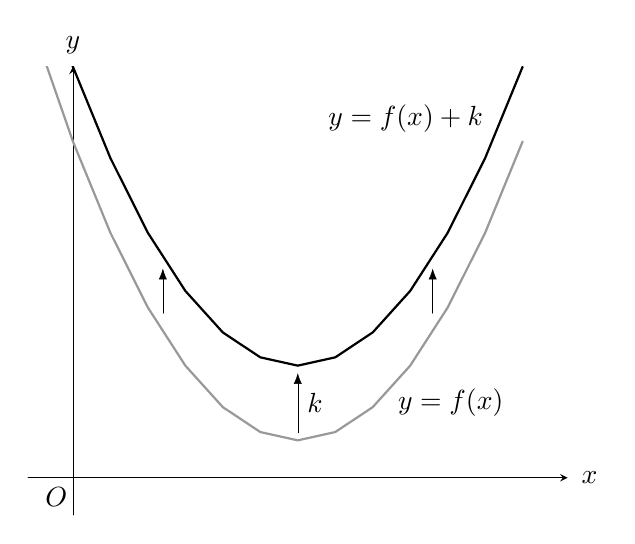
\begin{tikzpicture}
    \begin{axis}[
        axis lines=middle,
        xmin=-0.5, xmax=5.5,
        ymin=-0.5, ymax=5.5,
        xlabel={$x$},
        ylabel={$y$},
        ticks=none,
        xlabel style={anchor=east, xshift=0.5cm},
        ylabel style={anchor=north, yshift=0.5cm},
        line style={thick, color=black},
      ]
      \addplot[domain=-5:5, thick, color=black!40] {(0.8*x-2)^2 + 0.5};
      \addplot[domain=-5:5, thick] {(0.8*x-2)^2 + 1.5};
      \path (axis cs:0,0)
      node [anchor=north east, xshift=0.05cm] {$O$};
      \draw[-Latex] (axis cs:2.5, 0.6) -- (axis cs:2.5, 1.4) node [midway, right] {$k$};
      \draw[-Latex] (axis cs:1, 2.2) -- (axis cs:1, 2.8);
      \draw[-Latex] (axis cs:4, 2.2) -- (axis cs:4, 2.8);
      \node at (axis cs:3.7, 4.8) {$y = f(x) + k$};
      \node at (axis cs:4.2, 1) {$y = f(x)$};
    \end{axis}
  \end{tikzpicture}
  \hspace{1cm}
  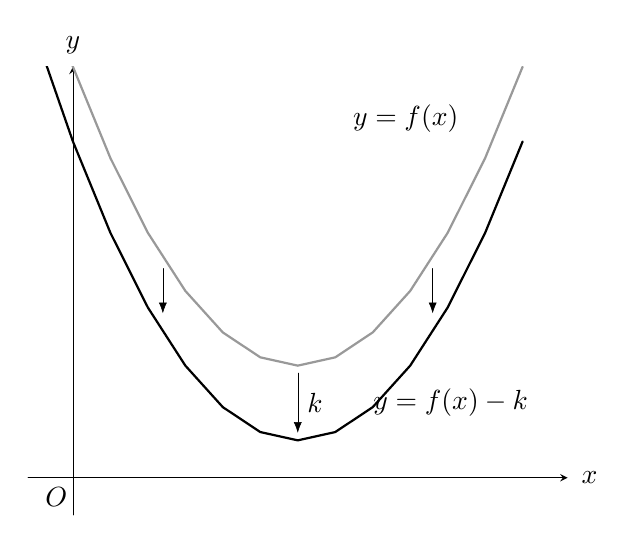
\begin{tikzpicture}
    \begin{axis}[
        axis lines=middle,
        xmin=-0.5, xmax=5.5,
        ymin=-0.5, ymax=5.5,
        xlabel={$x$},
        ylabel={$y$},
        ticks=none,
        xlabel style={anchor=east, xshift=0.5cm},
        ylabel style={anchor=north, yshift=0.5cm},
        line style={thick, color=black},
      ]
      \addplot[domain=-5:5, thick] {(0.8*x-2)^2 + 0.5};
      \addplot[domain=-5:5, thick, color=black!40] {(0.8*x-2)^2 + 1.5};
      \path (axis cs:0,0)
      node [anchor=north east, xshift=0.05cm] {$O$};
      \draw[-Latex] (axis cs:2.5, 1.4) -- (axis cs:2.5, 0.6) node [midway, right] {$k$};
      \draw[-Latex] (axis cs:1, 2.8) -- (axis cs:1, 2.2);
      \draw[-Latex] (axis cs:4, 2.8) -- (axis cs:4, 2.2);
      \node at (axis cs:3.7, 4.8) {$y = f(x)$};
      \node at (axis cs:4.2, 1) {$y = f(x) - k$};
    \end{axis}
  \end{tikzpicture}

\end{center}

\begin{mdframed}[style=MyFrame]
  \begin{itemize}[leftmargin=0.3cm]
    \item If $h > 0$, translate the graph of $y = f(x)$ horizontally to the right by $h$
          units, the graph of $y = f(x + h)$ is obtained.

    \item If $h > 0$, translate the graph of $y = f(x)$ horizontally to the left by $h$
          units, the graph of $y = f(x - h)$ is obtained.
  \end{itemize}
\end{mdframed}

\begin{mdframed}[style=MyFrame]
  \begin{itemize}[leftmargin=0.3cm]
    \item If $k > 0$, reflect the graph of $y = f(x)$ about the $x$-axis, the graph of $y
            = -f(x)$ is obtained.

    \item If $k > 0$, reflect the graph of $y = f(x)$ about the $y$-axis, the graph of $y
            = f(-x)$ is obtained.
  \end{itemize}
\end{mdframed}

\begin{mdframed}[style=MyFrame]
  If $a > 0$, zooming (when $a > 1$) or shrinking (when $0 < a < 1$) the graph of $y = f(x)$ by a factor of $a$ in the $y$-direction, the graph of $y = af(x)$ is obtained.
\end{mdframed}

\begin{mdframed}[style=MyFrame]
  If $a > 0$, shrinking (when $a > 1$) or zooming (when $0 < a < 1$) the graph of $y = f(x)$ by a factor of $\dfrac{1}{a}$ in the $x$-direction, the graph of $y = f(ax)$ is obtained.
\end{mdframed}

\subsection*{Practice 4}

\setlength{\columnseprule}{1pt}
\setlength{\columnsep}{24pt}

\begin{multicols}{2}

  Find the line of symmetry and vertex of the following parabola, and sketch its
  graph. (Question 1 to 2):
  \begin{enumerate}
    \item $y = 2x^2 + 8x + 11$
    \item $y = -3x^2 + 18x - 7$
  \end{enumerate}

  Sketch the graph of the following functions. (Question 3 to 4):
  \begin{enumerate}
    \setcounter{enumi}{2}
    \item $y = \dfrac{4}{{(x+2)}^2}$
    \item $y = \sqrt{x - 1} + 3$
  \end{enumerate}

\end{multicols}

\setlength{\columnseprule}{1pt}
\setlength{\columnsep}{24pt}

\subsection*{Exercise 22.3}

\begin{multicols}{2}

  Find the line of symmetry and vertex of the following parabola, and sketch its
  graph.
  \begin{enumerate}
    \item $y = 2x^2 + 4x + 5$
    \item $y = -3x^2 + 12x - 4$
    \item $y = 4x^2 - 20x + 19$
    \item $y = -3x^2 - 6x - 4$
  \end{enumerate}

  Sketch the graph of the following functions.
  \begin{enumerate}
    \setcounter{enumi}{4}
    \item $y = (x+2)^3 - 5$
    \item $y = \sqrt{x-5}$
    \item $y = \dfrac{1}{(x+2)^2}$
    \item $y = -\dfrac{1}{2(x-1)^2}$
    \item $y = 3\sqrt{x+1} - 4$
    \item $y = \dfrac{4}{2x+3}$
    \item $y = \left\{\begin{array}{ll}
              4x+9,   & x \leq 0 \\
              9 - 2x, & x > 0    \\
            \end{array}\right.$
    \item $y = \left\{\begin{array}{ll}
              \ \ \ \ \ \ \ \ \ \ x, & x < -1    \\
              \sqrt{x+1},            & x \geq -1 \\
            \end{array}\right.$
  \end{enumerate}

  \begin{enumerate}
    \setcounter{enumi}{12}
    \item Sketch the graph for the function $f(x) = x^2 - 6x + 12$, $-2 \leq x \leq 8$,
          and find its domain and range.
    \item Sketch the graph for the function $g(x) = -x^2 - 4x - 7$, $-2 \leq x \leq 5$,
          and find its domain and range.
    \item Sketch the graph for the function $f(x) = -x^2 + 2x + 10$, and find its domain
          and range.
    \item Sketch the graph of the function $y = \sqrt{x}$, and transform it according the
          following steps. Sketch the graph of each function after each step on the same
          diagram, and write down the corresponding function.

          Step 1: Translate 4 units to the left;

          Step 2: Scale up by a factor of 2 in the $x$-direction;

          Step 3: Reflect about the $y$-axis;

          Step 4: Translate 3 units downwards.

          Step 5: Scale down by half in the $y$-direction.
  \end{enumerate}

\end{multicols}

\section{Composite Functions}

Let $A$, $B$, and $C$ be three non-empty sets, $f: A \to B$ and $g: B \to C$ be
two functions, an element $x$ in set $A$ is mapped to an element $f(x)$ in set
$B$ by function $f$, and $f(x)$ is mapped to an element $g\big(f(x)\big)$ in
set $C$ by function $g$. In other words, $x$ in set $A$ is mapped to an element
$g\big(f(x)\big)$ in $C$ after two mappings. That is:
\begin{cequation}
  x\ \xrightarrow{\displaystyle \ \ f\ \ } f(x)\ \xrightarrow{\displaystyle \ \ g\ \ } g\big(f(x)\big)
\end{cequation}

The combination of these two mappings are a function from set $A$ to set $C$,
this function is called the \emph{composite function} of $f$ and $g$, denoted
by $g \circ f$. When defining the composite function $g \circ f$, the range of
$f$ must be a subset of the domain of $g$, that is, $R_f \subseteq D_g$.

Note that $D_{g \circ f} = D_f$, $R_{g \circ f} \subseteq R_g$.

$\forall n \in \mathbb{N}$, $f^{n+1} = f \circ f^n$.

Generally speaking, $g \circ f \neq f \circ g$.

If $f \circ (g \circ h)$ is defined, then $(f \circ g) \circ h$ is also
defined, and $f \circ (g \circ h) = (f \circ g) \circ h$. Therefore, we can
write $f \circ g \circ h$ without ambiguity.

\subsection*{Practice 5}

\setlength{\columnseprule}{1pt}
\setlength{\columnsep}{24pt}

\begin{multicols}{2}

  \begin{enumerate}[label=\arabic*., leftmargin=*]
    \item Let $f: \mathbb{R} \to \mathbb{R}$, $f(x) = 2x + 3$ and $g: \mathbb{R} \to
            \mathbb{R}$, $g(x) = 5 - x$. Find $(g \circ f)(x)$ and $(f \circ g)(x)$.

    \item Let $f: \mathbb{R} \to \mathbb{R}$, $f(x) = x^2 - 2x + 3$ and $g: \mathbb{R}
            \to \mathbb{R}$, $g(x) = 3x - 4$. Find
          \begin{enumerate}
            \item $g \circ f$ and $f \circ g$;
            \item $g\big(f(2)\big)$, $f\big(g(2)\big)$, $(g \circ f)(2)$, and $(f \circ g)(2)$.
          \end{enumerate}

    \item Let $f: \mathbb{R} \to \mathbb{R}$, $f(x) = 4 - x^2$ and $g: \left\{x | x \leq
            4 \right\} \to \mathbb{R}$, $g(x) = \sqrt{4 - x}$. Prove the existence of $f
            \circ g$ and $g \circ f$ respectively.
  \end{enumerate}

\end{multicols}

\section{One to One Function, Onto Function and One to One Onto Function}

\subsection*{One to One Function}

Let $f: A \to B$ be a function, if there is at most one preimage in set $A$ for
each element in set $B$, then $f$ is called a \emph{one to one function}.

As shown in the diagram above, each element in the codomain $B$ of the function
$f: A \to B$ has at most one preimage in the domain $A$ of the function, thus
$f$ is a one to one function; while the element $b_2$ in the codomain $B$ of
the function $g: A \to B$ has two preimages $a_2$ and $a_3$, thus $g$ is not a
one to one function.

A function $y = f(x)$ is a one to one function, if and only if any line
parallel to the $x$-axis intersects the graph of the function at most once.

\subsection*{Onto Function}

If each element in the codomain $B$ of the function $f: A \to B$ has at least
one preimage under the function $f$, then $f$ is said to be an \emph{onto
  function}.

As shown in the diagram above, each element in the codomain $B$ of the function
$f: A \to B$ has at least one preimage under the function $f$, therefore $f$ is
an onto function; while the element $b_3$ in the codomain $B$ of the function
$g: A \to B$ has no preimage under the function $g$, therefore $g$ is not an
onto function.

\subsection*{One to One Onto Function}

If a function is both a one to one function and an onto function, then it is a
\emph{one to one onto function}, as shown in the diagram above.

\subsection*{Practice 7}

Determine whether the following functions are one to one functions or onto
functions.

\subsection*{Exercise 22.5}

\setlength{\columnseprule}{1pt}
\setlength{\columnsep}{24pt}

\begin{multicols}{2}

  \begin{enumerate}
    \item Let $A = \left\{1, 2, 3\right\}$, $f: A \to A$ is defined by $f: 1 \to 1$, $2
            \to 3$, $3 \to 2$. Determine if $f$ is a one to one function or an onto
          function.

    \item Let $A = \left\{a, b, c, d\right\}$ and $B = \left\{x, y, z\right\}$, $f: A \to
            B$ is defined by $f: a \to y$, $b \to x$, $c \to z$, $d \to y$. Determine if
          $f$ is a one to one function or an onto function.

    \item Let the function $g: \mathbb{R} \to \mathbb{R}$ be defined by $g(x) = 2x + 1$.
          Determine if $g$ is a one to one function or an onto function.

    \item Let the function $f: \mathbb{R} \to \mathbb{R}$ be defined by $f(x) = 2x^3 -
            3$. Determine if $f$ is a one to one function or an onto function.

    \item Let the function $f: \mathbb{R}^+ \to \mathbb{R}^+$ be defined by $f(x) =
            \dfrac{1}{x}$. Determine if $f$ is a one to one function or an onto function.

    \item Let the function $f: \mathbb{R}^+ \to \mathbb{R}^+$ be defined by $f(x) =
            \sqrt{x}$. Determine if $f$ is a one to one function or an onto function.

    \item Determine whether the following functions are one to one, onto or one to one
          onto functions.
          \begin{enumerate}
            \item $A = \left\{a, b, c\right\}$, $B = \left\{x, y, z\right\}$, $f: A \to
                    B$, $f: a \to x$, $b \to x$, $c \to y$
            \item $A = \left\{a, b, c\right\}$, $B = \left\{x, y, z\right\}$, $g: A \to
                    B$, $g: a \to x$, $b \to y$, $c \to z$
            \item $A = \left\{a, b, c\right\}$, $B = \left\{x, y\right\}$, $h: A \to
                    B$, $h: a \to x$, $b \to y$, $c \to y$
            \item $A = \left\{a, b, c\right\}$, $B = \left\{x, y\right\}$, $k: A \to
                    B$, $k: a \to x$, $a \to y$, $c \to y$
            \item $A = \left\{a, b, c\right\}$, $B = \left\{x, y\right\}$, $f: A \to B$, $f: a \to x$, $a \to y$, $b \to x$, $c \to y$
            \item $A = \left\{a, b, c, d\right\}$, $B = \left\{u, v, x, y, z\right\}$, $g: A \to B$, $g: a \to u$, $b \to v$, $c \to x$, $d \to y$
          \end{enumerate}

    \item Determine whether the following functions mapping $A$ to $B$ are one to one
          functions or onto functions.
  \end{enumerate}

\end{multicols}

\newpage

\section{Inverse Functions}

\begin{mdframed}[style=MyFrame]
  If $f: A \to B$ is a one to one onto function, then there exist a function $g: B \to A$, such that if $y = f(x)$, then $g(y) = x$. The function $g$ is called the \emph{inverse function} of $f$, and is denoted by $f^{-1}$.
\end{mdframed}

from the diagram above, we can conclude the following:

\begin{mdframed}[style=MyFrame]
  \begin{cequation}
    x\ \xrightarrow{\displaystyle \ \ f\ \ } y = f(x)\ \xrightarrow{\displaystyle \ \ f^{-1}\ \ } f^{-1}\big(f(x)\big) = f^{-1}(y)
  \end{cequation}
\end{mdframed}
or
\begin{mdframed}[style=MyFrame]
  \begin{cequation}
    y\ \xrightarrow{\displaystyle \ \ f^{-1}\ \ } x = f^{-1}(y)\ \xrightarrow{\displaystyle \ \ f\ \ } f\big(f^{-1}(y)\big) = f(x)
  \end{cequation}
\end{mdframed}

If both $(g\circ f)^-1$ and $f^{-1} \circ g^{-1}$ exist, then $(g\circ f)^{-1}
  = f^{-1} \circ g^{-1}$.

\subsection*{Practice 8}

\subsection*{Exercise 22.5}

\setlength{\columnseprule}{1pt}
\setlength{\columnsep}{24pt}

\begin{multicols}{2}

  \begin{enumerate}
    \item Find the inverse function of the following functions:
          \begin{enumerate}
            \item $f:x \to 7x - 3$
            \item $g:x \to \dfrac{1}{2}x + 9$
            \item $h:x \to \dfrac{x+1}{x-8},\ x \neq 8$
            \item $k:x \to \dfrac{x-1}{2x},\ x \neq 0$
          \end{enumerate}

    \item Given the function $f: x \to 2x+1$ and $g:x \to \dfrac{1}{x-4},\ x\neq 4$.
          Find:
          \begin{enumerate}
            \item $f^{-1}$
            \item $g^{-1}$
            \item $f^{-1} \circ g^{-1}$
            \item $g^{-1} \circ f^{-1}$
            \item $(f \circ g)^{-1}$
            \item $(g \circ f)^{-1}$
          \end{enumerate}
  \end{enumerate}

\end{multicols}

\subsection*{Graph of Inverse Functions}

\begin{mdframed}[style=MyFrame]
  If $f$ is a one to one function, then the graph of $f^{-1}$ is the reflection of the graph of $f$ about the line $y = x$.
\end{mdframed}

\subsection*{Practice 9}

Given the function $g: \mathbb{R}^+ \cup {0} \to \mathbb{R}^+ \cup {0}$, $g: x
  \to x^2$. On the same set of axes, draw the graph of the function $g$ and its
inverse function $g^{-1}$.

\subsection*{Exercise 22.6}

\setlength{\columnseprule}{1pt}
\setlength{\columnsep}{24pt}

\begin{multicols}{2}

  \begin{enumerate}
    \item Find the inverse function of the following functions:
          \begin{enumerate}
            \item $f:x \to 2x - 7$
            \item $g:x \to \dfrac{1}{x-2},\ x \neq 2$
            \item $h:x \to \dfrac{2x - 5}{x-2},\ x \neq 2$
            \item $k:x \to \dfrac{3x}{x-4},\ x \neq 4$
          \end{enumerate}

    \item Given that $f:x \to \dfrac{160}{ax + b}$, $f(5) = 8$ and $f(9) = 10$. Find
          \begin{enumerate}
            \item the values of $a$ and $b$;
            \item $f^{-1}(16)$.
          \end{enumerate}

    \item Given that $f:x \to \dfrac{a}{x+b}$,\ $f(3) = -1$, and $f(-9) = 3$. Find
          \begin{enumerate}
            \item the values of $a$ and $b$;
            \item the value of $x$ such that $f(x) = f^{-1}(x)$.
          \end{enumerate}

    \item Given the function $g:x \to \dfrac{6}{x} - 3$,\ $x \neq 0$. Find
          \begin{enumerate}
            \item $g^{-1}$;
            \item the value of $x$ such that $g^{-1}(x) = x - 2$.
          \end{enumerate}

    \item Given the function $f:x \to ax + b$ and $f^2: x \to 4x + 12$. If $a > 0$, find
          \begin{enumerate}
            \item the values of $a$ and $b$;
            \item $f^{-1}(3)$.
          \end{enumerate}

    \item Given the function $f:x \to 3x - 2$ and $g:x \to \dfrac{x}{x+4}$, $x \neq -4$.
          Find
          \begin{enumerate}
            \item $f^{-1}$
            \item $g^{-1}$
            \item $f^{-1} \circ g^{-1}$
            \item $g^{-1} \circ f^{-1}$
            \item $(f \circ g)^{-1}$
            \item $(g \circ f)^{-1}$
          \end{enumerate}

    \item Given the function $f: \mathbb{R} \setminus \{2\} \to \mathbb{R} \setminus
            \{0\}$, $f:x \to \dfrac{1}{x-2}$.
          \begin{enumerate}
            \item Find $f^{-1}$.
            \item On the same set of axes, draw the graph of $f$ and $f^{-1}$.
          \end{enumerate}

    \item Given the function $f:x \to 2\sqrt{x+4}$, $x \geq -4$,
          \begin{enumerate}
            \item Find $f^{-1}$.
            \item On the same set of axes, draw the graph of $f$ and $f^{-1}$.
          \end{enumerate}
  \end{enumerate}

\end{multicols}

\subsection*{Revision Exercise 22}

\setlength{\columnseprule}{1pt}
\setlength{\columnsep}{24pt}

\begin{multicols}{2}
  \begin{enumerate}
    \item Determine whether the following mappings from set $A = \{1, 2, 3, 4\}$ to set
          $B = \{a, b, c, d\}$ are functions or not.
          \begin{enumerate}
            \item $1 \to a$, $2 \to c$, $4 \to b$
            \item $1 \to a$, $2 \to d$, $3 \to b$, $4 \to a$
            \item $1 \to c$, $2 \to c$, $3 \to b$, $4 \to b$
            \item $1 \to a$, $2 \to c$, $2 \to b$, $4 \to d$
            \item $1 \to c$, $2 \to b$, $3 \to d$, $4 \to c$, $4 \to a$
          \end{enumerate}

    \item Given the function $f: \mathbb{R} \to \mathbb{R}$ be defined by $f(x) = \left\{\begin{array}{rl}
              3x - 2,   & x < -3        \\
              2x^2 + 4, & -3 \leq x < 2 \\
              -2x + 9,  & x \geq 2
            \end{array}\right.$, find
          \begin{enumerate}
            \item $f(-4)$
            \item $f(0)$
            \item $f(2)$
            \item $f(3)$
          \end{enumerate}

    \item Find the domain and range of the following functions:
          \begin{enumerate}
            \item $f: 1 \to 3$, $2 \to 5$, $4 \to 8$
            \item $g: 2 \to 4$, $4 \to 5$, $5 \to 7$, $6 \to 9$
            \item $h: 1 \to 3$, $2 \to 5$, $3 \to 6$, $4 \to 8$
          \end{enumerate}

    \item The table below shows a function $f$:
          \begin{center}
            \begin{tabular}{|c|c|c|c|c|c|}
              \hline
              x    & -3  & -2 & -1 & 0 & 1 \\
              \hline
              f(x) & -22 & -3 & 4  & 5 & 6 \\
              \hline
            \end{tabular}
          \end{center}
          \begin{enumerate}
            \item Find the domain and range of the function;
            \item Sketch the graph of the function.
            \item Determine if the inverse function of $f$ exists.
          \end{enumerate}

    \item As shown in the diagram below, let a function $f: x \to ax + b$. Find the value
          of $f(4)$ and $f^{-1}(5)$.

    \item Given the function $f:x \to x^2 - x + 1$, $-1 \leq x \leq 3$, find its range.

    \item Let function $f:x \to 2x^2 - 4x + 3$.
          \begin{enumerate}
            \item If $D_f = \mathbb{R}$, find the range of $f$;
            \item If $D_f = \big\{x | x \geq 3\big\}$, find the range of $f$.
          \end{enumerate}

    \item Find the domain and range of the following functions:
          \begin{enumerate}
            \item $f(x) = \dfrac{1}{x}$
            \item $f(x) = \sqrt{2x - 5}$
            \item $f(x) = x^2 + 4x + 7$
            \item $f(x) = \dfrac{1}{x^2 + 4}$
          \end{enumerate}

    \item Find the domain of the following functions:
          \begin{enumerate}
            \item $f(x) = \dfrac{2x}{x-3}$
            \item $f(x) = \sqrt{4 - x^2}$
            \item $f(x) = \dfrac{x-2}{2x^2 - 5x + 2}$
            \item $f(x) = \dfrac{x-3}{\sqrt{x^2 - 9}}$
          \end{enumerate}

    \item Sketch the graph for the following functions:
          \begin{enumerate}
            \item $f(x) = 2x^2 - 5x + 9$
            \item $f(x) = -3x^2 + 6x + 11$
            \item $f(x) = 3x^2 + 12x + 10$
            \item $f(x) = -5x^2 + 6x + 11$
            \item $f(x) = 2x^3 - 7$
            \item $f(x) = \sqrt{3x - 9}$
            \item $f(x) = \dfrac{4}{2x+11}$
            \item $f(x) = \dfrac{2x + 7}{x-1}$
            \item $f(x) = 2\sqrt{x+5} - 4$
            \item $f(x) = \dfrac{1}{(2x - 3)^2}$
            \item $f(x) = \left\{\begin{array}{rl}
                      2x + 1, & x < 0    \\
                      x^2,    & x \geq 0
                    \end{array}\right.$
            \item $f(x) = \left\{\begin{array}{rl}
                      1 - x^2,      & x \leq 1 \\
                      x^2 + 2x - 3, & x > 1
                    \end{array}\right.$
          \end{enumerate}

    \item Given the function $f:x \to 2x^2$ and $g:x \to 3x - 4$. Find the value of $m$
          such that $(f \circ g)(m) = (g \circ f)(m)$.

    \item Given the function $f:x \to x^2 + 2x - 3$ and $g:x \to 3x - 4$. If $(f \circ
            g)(k) = (g \circ f)(k)$, find the value of $k$.

    \item Given that $f(x) = 3x + 1$, $x \neq 0$. If $(f \circ g)(x) = 6x^2 - 9x + 4$,
          find $g(x)$.

    \item Given that $f(x) = \dfrac{x+1}{x}$, $x \neq 0$. IF $(f \circ g)(x) = x$, find
          $g(x)$.

    \item A function $f$ is defined by $f: x \to x - 3$. Find another function $g$ such
          that $g\circ f: x\to 4x^2 - 20x + 25$.

    \item Let $f: \mathbb{R} \to \mathbb{R}$ be defined by $f(x) = \left\{\begin{array}{rl}
              -2,       & x\leq -3   \\
              |x| - 2x, & -3 < x < 3 \\
              2x - 1,   & x \geq 3
            \end{array}\right.$. Find $(f \circ f \circ f)(-1000).$

    \item Let function $f: A \to \mathbb{R}$ be defined by $f: x \to 2x^2$. Determine if
          $f$ is one to one function when $A$ is the following sets.
          \begin{enumerate}
            \item $A = \big\{x | 0 \leq x < 6\big\}$
            \item $A = \big\{x | x < 0\big\}$
            \item $A = \big\{x | -2 \leq x < 2\big\}$
            \item $A = \big\{x | x > 3\big\}$
          \end{enumerate}

    \item Determine whether the following functions are one to one functions or onto
          functions.
          \begin{enumerate}
            \item $f: \mathbb{R}^+ \to \mathbb{R}$, $f:x \to |x|-2$
            \item $f: \mathbb{R}\setminus\big\{2\big\} \to \mathbb{R}\setminus\big\{1\big\}$, $f:x \to \dfrac{x}{x-2}$
            \item $f: \mathbb{R} \to \mathbb{R}^+\cup\big\{0\big\}$, $f:x \to |x|$
          \end{enumerate}

    \item Let $A = \mathbb{R} \setminus \left\{-\dfrac{1}{2}\right\}$ and $A = \mathbb{R}
            \setminus \left\{\dfrac{1}{2}\right\}$, function $f: A \to B$ is defined by
          $f(x) = \dfrac{x-3}{2x + 1}$. Find
          \begin{enumerate}
            \item $f^{-1}(-2)$
            \item $f^{-1}(0)$
            \item $f^{-1}(3)$
          \end{enumerate}

    \item Let function $f: \mathbb{R}^+ \to \mathbb{R}^+$ be defined by $f(x) = x^2 + 2x
            + 1$. Find $f^{-1}(4)$ and $f^{-1}(9)$.

    \item A function $f$ is defined by $f:x \to \dfrac{x}{2} + 1$. If $g \circ f^{-1}: x
            \to 4x^2 - 8x + 7$, find the function $g$.

    \item Given the functioon $f:x \to 3x^2 + 5x + 9$, $x \leq a$. Find the maximum value
          of $a$ such that the inverse function of $f$ exists.

    \item Let the function $f$ and $g$ be defined as $f:x \to 5x + 3$ and $g:x \to 2x -
            7$ respectively. Find
          \begin{enumerate}
            \item $f \circ g$
            \item $f^{-1}$
            \item $g^{-1}$
          \end{enumerate}

    \item Given the function $f:x \to 2x + 3$ and $g:x \to {3-x}{2x + 5}$, $x \neq
            -\dfrac{5}{2}$. Find
          \begin{enumerate}
            \item $f \circ g$
            \item $f^{-1}$
            \item $g^{-1}$
          \end{enumerate}
          Show that $g^{-1} \circ f^{-1} = (f \circ g)^{-1}$.

    \item Given the function $f:x \to \sqrt{x}$, $x \neq 0$ and $g:x \to x^3$. Find
          \begin{enumerate}
            \item $g \circ f$
            \item $f^{-1}$
            \item $g^{-1}$
            \item $(g \circ f)^{-1}$
            \item $g^{-1} \circ f^{-1}$
          \end{enumerate}

    \item Given the function $f:x \to 2\sqrt{x-4} + 3$, $x \geq 4$.
          \begin{enumerate}
            \item Find the range of $f$.
            \item Find the inverse function $f^{-1}$ of $f$.
            \item On the same diagram, sketch the graphs of $f$ and $f^{-1}$.
          \end{enumerate}

  \end{enumerate}
\end{multicols}

\chapter{Exponents and Logarithms}

\section{Exponents}

\subsection*{Definition and Properties of Exponents}

Back in Junior 1, we have learnt the following definitions of exponents:
\begin{flalign*}
  \text{\textbf{Positive exponent}\ \ \ \ \ \ \ }   & a^n = \underbrace{a \times a \times \cdots \times a}_{n \text{ times}}                                 & \\
  \text{\textbf{Zero exponent}\ \ \ \ \ \ \ }       & a^0 = 1                                                                                                & \\
  \text{\textbf{Negative exponent}\ \ \ \ \ \ \ }   & a^{-n} = \dfrac{1}{a^n}\ (a \neq 0, n \in \mathbb{Z}^+)                                                & \\
  \text{\textbf{Fractional exponent}\ \ \ \ \ \ \ } & a^{\frac{m}{n}} = \left(\sqrt[n]{a}\right)^m = \sqrt[n]{a^m}\ (a \geq 0, n > 1, m, n \in \mathbb{Z}^+) &
\end{flalign*}

\noindent The exponent of rational numbers have the following properties:
\begin{enumerate}
  \item $a^m \times a^n = a^{m+n}$
  \item $\dfrac{a^m}{a^n} = a^{m-n}$
  \item $\left(a^m\right)^n = a^{mn}$
  \item $\left(ab\right)^n = a^nb^n$
  \item $\left(\dfrac{a}{b}\right)^n = \dfrac{a^n}{b^n}\ (b \neq 0)$
\end{enumerate}

\subsection*{Practice 1}

Without using the calculator, find the value of the following expressions
(Question 1 to 2):
\begin{enumerate}
  \item $2^{-2} + 2{-5} - (-2)^{-3}$
  \item $\left(3\dfrac{6}{25}\right)^{-\frac{1}{2}}$
  \item Simplify $a^-4 \div a^{-5} \times (b^{-3})^{-4}$
\end{enumerate}

\subsection*{Exponential Functions and Graphs}

Let $a$ is a constant that is bigger than zero and not equal to 1, then the
function being expressed in the form of $y = a^x$ is called an
\emph{exponential function}. The domain of an exponential function is
$\mathbb{R}$.

Consider the following: a cell divides into two cells, and then each of the two
cells divides into two cells again, and so on. If we let $x$ be the number of
divisions, the number of cells after the divisions be $y$, then the functional
relationship between $x$ and $y$ is $y = 2^x$, which is an exponential
function.

In order to look into the graph and its properties of an exponential function
$y = a^x$, we sketch the graph of some exponential functions, the graph of $y =
  2^x$, $y = 10^x$, and $y = \left(\dfrac{1}{2}\right)^x$ are shown in the
diagram below.

From the diagram above, we can see that:
\begin{enumerate}[label=(\arabic*)]
  \item The graph of the function $y = 2^x$, $y = 10^x$, and $y =
          \left(\dfrac{1}{2}\right)^x$ are only at the top of the $x$-axis. Actually,
        when $a > 0$, $a^x > 0$. Therefore, the value of the exponential function $y =
          a^x$ is always positive.

  \item When $x = 0$, $y = 1$. Hence, the graph of exponential functions $y = a^x$
        always passes through the point $(0, 1)$.

  \item For the function $y = 2^x$, when $x > 0$ and $y = 10^x$, when $x < 0$, $y < 1$;
        when $x > 0$, $y > 1$. When the value of $x$ increases, the value of $y$
        increases, that is, the function is an increasing function in the interval
        $(-\infty, +\infty)$.

  \item For the function $y = \left(\dfrac{1}{2}\right)^x$, when $x > 0$, $y > 1$; when
        $x < 0$, $y < 1$. When the value of $x$ increases, the value of $y$ decreases,
        that is, the function is a decreasing function in the interval $(-\infty,
          +\infty)$.
\end{enumerate}

When we are discussing about the graph and its properties of an exponential
function $y = a^x$, the following two cases are considered: \newpage

\subsection*{Practice 2}

\setlength{\columnseprule}{1pt}
\setlength{\columnsep}{24pt}

\begin{multicols}{2}
  \begin{enumerate}
    \item Without using the calculator, compare the value of the following expressions:
          \begin{enumerate}
            \item $\pi^{2.1}$ and $\pi^{3.5}$
            \item $0.5^{-2.3}$ and $0.5^{-3.8}$
          \end{enumerate}

    \item Given the exponential functions $f(x) = 3^{x^2 - 3x + 5}$ and $g(x) =
            3^{x+10}$. Find the value of $x$ such that $f(x) = g(x)$.
  \end{enumerate}
\end{multicols}

\subsection*{Exercise 23.1}

\setlength{\columnseprule}{1pt}
\setlength{\columnsep}{24pt}

\begin{multicols}{2}
  Without using the calculator, find the value of the following expressions (Question 1 to 10):
  \begin{enumerate}
    \item $\left(\dfrac{1}{3}\right)^2 + \left(\dfrac{1}{3}\right)^0 - \left(-\dfrac{1}{3}\right)^{-2}$
    \item $\left(\dfrac{3^{-5}\cdot3^{2}}{3^{-3}}\right)^{-2}$
    \item $6^{-8} \div 6^{-5} + 3^{-3}$
    \item $12^{\frac{1}{3}} \times 6^{\frac{1}{3}} \div 27^{\frac{1}{6}} \div 3^{\frac{1}{6}}$
    \item $(0.2)^{-2}\times (0.125)^{\frac{2}{3}}$
    \item $(0.3)^{-\frac{1}{3}}\times(0.0081)^{\frac{1}{3}}+(0.064)^{\frac{1}{3}}$
    \item $\left(\dfrac{81}{16}\right)^{-\,0.25}\times\left(\dfrac{8}{27}\right)^{-\frac{2}{3}}\times(0.25)^{-2.5}$
    \item $\left(\frac{1}{2}\right)^{-2}+125^{\frac{2}{3}}+343^{\frac{1}{3}}-\left(\dfrac{1}{27}\right)^{-\frac{1}{3}}$
    \item $\left(2{\dfrac{1}{4}}\right)^{-{\frac{3}{2}}}+\left(1{\dfrac{11}{25}}\right)^{-1}-\left(2{\dfrac{2}{3}}\right)^{0}$
    \item $\dfrac{5\sqrt{4}\sqrt{8}\left({\sqrt[3]{\sqrt[5]{4}}}\right)^{2}}{\sqrt[3]{\sqrt{2}}}$
  \end{enumerate}

  \noindent Simplify the follwoing expressions (Question 11 to 24):
  \begin{enumerate}
    \setcounter{enumi}{10}
    \item $a^{\frac{1}{2}}\cdot a^{\frac{1}{4}}\cdot a^{-{\frac{1}{8}}}\cdot a^{\frac{1}{6}}$
    \item $\left(9a^{2}b^{-2}c^{4}\right)^{-1}$
    \item $\left(x^{4}y^{-5}\right)\left(x^{-2}y^{2}\right)^{2}$
    \item $3a^{-2}b^{-3}\div\left(-3^{-1}a^{2}b^{-3}\right)$
    \item $\sqrt[3]{\dfrac{a^{2}b^{-1}}{a^{\frac{1}{2}}b^{5}}}$
    \item $5a^{-2}b^{-3}\div\left(5^{-1}a^{2}b^{-3}\right)\times 5^{-2}a b^{4}c$
    \item $\dfrac{a^{-2}-b^{-2}}{a^{-2}+b^{-2}}$
    \item $\left(a^{-1}+b^{-1}\right)\left(a+b\right)^{-1}$
    \item $\left(x+x^{-1}\right)\left(x-x^{-1}\right)$
    \item $\left(-2x^{\frac{1}{4}}y^{-\frac{1}{3}}\right)\left(3x^{-\frac{1}{2}}y^{\frac{2}{3}}\right)\left(-4x^{\frac{1}{4}}y^{\frac{2}{3}}\right)$
    \item $2x^{-{\frac{1}{3}}}\left({\dfrac{1}{2}}x^{{\frac{1}{3}}}-2x^{-{\frac{2}{3}}}\right)$
    \item $\left(\sqrt{x^{3}}\cdot\sqrt{y}\right)^{2}\cdot\left(\sqrt{y}\cdot\sqrt{x^{3}}\right)^{3}$
    \item $\dfrac{3\times2^{n}-4\times2^{n-2}}{2^{n}-2^{n-1}}$
    \item $\left(3^{n+6}-5\times3^{n+1}\right)\div\left(7\times3^{n+2}\right)$
    \item Sketch the graph of the following functions on the same diagram:
          \begin{enumerate}[label=(\alph*)]
            \item $y = 3^x$
            \item $y = \left(\dfrac{1}{3}\right)^x$
          \end{enumerate}
    \item Without using the calculator, compare the value of the following expressions:
          \begin{enumerate}
            \item $2.5^{7.1}$ and $2.5^{8.5}$
            \item $0.35^{6.5}$ and $0.35^{5.6}$
            \item $1.03^{-2.1}$ and $1.03^{-3.2}$
            \item $\left(\sqrt{2}\right)^\pi$ and $\left(\sqrt{2}\right)^{\pi - 3.5}$
            \item $0.01^{-\frac{1}{3}}$ and $0.01^{-\frac{1}{2}}$
            \item $2.7^{\sqrt{20}}$ and $2.7^{\sqrt[3]{35}}$
          \end{enumerate}

    \item Given that $f_1: x \to 2^{3x}$ and $f_2: x \to 2^{x^2 + 2}$. Find the value of
          $x$ such that $f_1(x) = f_2(x)$.

    \item Given the function $f(x) = (0.4)^{x^2 - x + 1}$ and $g(x) = (0.4)^{6x + 19}$.
          Find the value of $x$ such that $f(x) = g(x)$.
  \end{enumerate}

\end{multicols}

\section{Logarithms}

\subsection*{Definition of Logarithms}

If $a_n = x$, where $a > 0$ and $a \neq 1$, then we define $\log_a x = n$, and
we say that $n$ is the logarithm of $x$ to the base $a$. In $\log_a x$, $a$ is
called the base, $x$ is called the antilogarithm.

On the other hand, if $\log_a x = n$, then $a_n = x$. This is the inversible
relationship between exponents and logarithms. That is,
\begin{mdframed}[style=MyFrame]
  \vspace{-10pt}
  \begin{cequation}
    \log_a x = n \iff a^n = x\qquad
    a > 0,\ a \neq 1,\ x > 0
  \end{cequation}
\end{mdframed}

Logarithms with base $10$ are called common logarithms, and are usually written
as $\log a$.

Another common logarithm is the natural logarithm, which has base $e$ ($e
  \approx 2.71828182846$), and is usually written as $\ln x$.

\subsection*{Practice 3}

Find the value of $x$ in the following equations:

\setlength{\columnseprule}{1pt}
\setlength{\columnsep}{24pt}

\begin{multicols}{2}
  \begin{enumerate}
    \item $\log x = 3$
    \item $\log_x 27 = \dfrac{3}{2}$
    \item $2\log_x(3\sqrt{3}) = 1$
    \item $\log_2(16\sqrt{2}) = x$
  \end{enumerate}
\end{multicols}

\subsection*{Logarithmic Functions and Graphs}

From the definition of logarithms, we can see that if $y = a^x$, then $x =
  \log_a y$. From the concept of inverse functions, we know that $y = \log_a x$
is the inverse function of $y = a^x$. Function $y = \log_a x$ is called the
logarithmic function, where $a > 0$ and $a \neq 1$. Since the domain of $y =
  a^x$ is $\mathbb{R}$, and its range is $\mathbb{R}^+$, so the domain of $y =
  \log_a x$ is $\mathbb{R}^+$, and its range is $\mathbb{R}$.

Since the logarithmic function $y = \log_a x$ is the inverse function of the
exponential function $y = a^x$, so the graph of $y = \log_a x$ is the
reflection of the graph of $y = a^x$ about the line $y = x$. If we draw a curve
of $y = a^x$, then reflect it about the line $y = x$, we can get the graph of
$y = \log_a x$. For example, in the diagram below, the curves that are the
reflection of the graphs of $y = 2^x$ and $y = \left(\dfrac{1}{2}\right)^x$
about the line $y = x$ are the graphs of $y = \log_2 x$ and $y =
  \log_\frac{1}{2} x$ respectively.

From the diagram above, we can see that:
\begin{enumerate}[label=(\arabic*)]
  \item Since the domain of $y = \log_a x$ is $x > 0$, so the graph of the function $y
          = \log_2 x$ and $y = \log_\frac{1}{2} x$ are only at the right side of the
        $y$-axis.
  \item When $x = 1$, $y = 0$. Hence, the graph of logarithmic functions $y = a^x$
        always passes through the point $(1, 0)$.

  \item For the function $y = \log_2 x$, when $x > 1$, $y > 0$; when $0 < x < 1$, $y <
          0$. When the value of $x$ increases, the value of $y$ increases, that is, the
        function is an increasing function in the interval $(0, +\infty)$.

  \item For the function $y = \log_\frac{1}{2} x$, when $x > 1$, $y < 0$; when $0 < x <
          1$, $y > 0$. When the value of $x$ increases, the value of $y$ decreases, that
        is, the function is a decreasing function in the interval $(0, +\infty)$.
\end{enumerate}

When we are discussing about the graph and properties of a logarithmic function
$y = \log_a x$, the following two cases are considered: \newpage

\subsection*{Practice 4}

\setlength{\columnseprule}{1pt}
\setlength{\columnsep}{24pt}

\begin{multicols}{2}
  \begin{enumerate}
    \item Without using the calculator, Compare the value of the following expressions:
    \item \begin{enumerate}
            \item $\log 6$ and $\log 9$
            \item $\log_{0.5} 4.2$ and $\log_{0.5} 3.9$
            \item $\log_2 1.8$ abd $\log_4 5.8$.
          \end{enumerate}
    \item Find the domain of the following functions:
          \begin{enumerate}
            \item $y = \log_a(x+2)$
            \item $y = \log_2(x^2 - 9)$
            \item $y = \log_7\dfrac{2}{3-2x}$
            \item $y - \sqrt{\log_5(2-x)}$
          \end{enumerate}
  \end{enumerate}
\end{multicols}

\subsection*{Exercise 23.2}

\setlength{\columnseprule}{1pt}
\setlength{\columnsep}{24pt}

\begin{multicols}{2}
  \begin{enumerate}
    \item Find the value of $x$ for the following expression:
          \begin{enumerate}
            \item $\log_2 x = 4$
            \item $\log_{125} x = \dfrac{1}{3}$
            \item $\log_{16}(2\sqrt{2}) = x$
            \item $\log_\frac{1}{3}81 = x$
            \item $\log_x 81 = 4$
            \item $\log_x 49 = -2$
          \end{enumerate}

    \item Sketch the graph of the following functions on the same set of axes:
          \begin{enumerate}
            \item $y = \log_5 x$
            \item $y = \log_\frac{1}{5} x$
          \end{enumerate}

    \item Without using the calculator, compare the value of the following expressions:
          \begin{enumerate}
            \item $\log_3 5$ and $\log_3 6$
            \item $\log{1.5} 1.4$ and $\log_{1.5} 1.6$
            \item $\log_{\sqrt{3}} 4.8$ and $\log_{\sqrt{3}} 5.8$
            \item $\log_{2.3} \pi$ and $\log_{2.3} (\pi - 3)$
            \item $\log_{0.4}\sqrt{2}$ and $\log_{0.4}\sqrt{3}$
            \item $\log_\frac{1}{2} 3$ and $\log_\frac{1}{2} \dfrac{1}{4}$
          \end{enumerate}

    \item Find the domain of the following functions:
          \begin{enumerate}
            \item $y = \log_2 (3-2x)$
            \item $y = \log(x^2 + 1)$
            \item $y = \log_5(9-16x^2)$
            \item $y = \log_9 \dfrac{1}{x-2}$
            \item $y = \log_8 \sqrt{2x^2 - x - 3}$
            \item $y = \dfrac{1}{\log_3 (7x-5)}$
          \end{enumerate}
  \end{enumerate}
\end{multicols}

\section{Arithmetic Properties of Logarithms and Base Changing Formula}

\subsection*{Identties and Arithmetic Properties of Logarithms}

Logarithms have the following identities:
\begin{mdframed}[style=MyFrame]
  \setlength{\abovedisplayshortskip}{0pt}
  \setlength{\belowdisplayshortskip}{0pt}
  \setlength{\abovedisplayskip}{0pt}
  \setlength{\belowdisplayskip}{0pt}
  \makeatletter
  \setbool{@fleqn}{false}
  \makeatother
  \begin{flalign*}
    \log_a 1 & = 0 \\
    \log_a a & = 1
  \end{flalign*}
  \makeatletter
  \setbool{@fleqn}{true}
  \makeatother
\end{mdframed}

\noindent Logarithms have the following arithmetic properties:
\begin{mdframed}[style=MyFrame]
  \setlength{\abovedisplayshortskip}{0pt}
  \setlength{\belowdisplayshortskip}{0pt}
  \setlength{\abovedisplayskip}{0pt}
  \setlength{\belowdisplayskip}{0pt}
  \makeatletter
  \setbool{@fleqn}{false}
  \makeatother
  \begin{flalign*}
     & \log_a(xy) = \log_a x + \log_a y \quad (x > 0, y > 0)          \\
     & \log_a \dfrac{x}{y} = \log_a x - \log_a y \quad (x > 0, y > 0) \\
     & \log_a x^n = n \log_a x \quad (x > 0)                          \\
     & a^{\log_a x} = x
  \end{flalign*}
  \makeatletter
  \setbool{@fleqn}{true}
  \makeatother
\end{mdframed}

\subsection*{Base Changing Formula}

The base of a logarithm can be changed from one to another. Let $\log_a x = n$,
then $a^n = x$. Change both sides of the equation to logarithm with base $b$,
we have
\begin{flalign*}
  \log_b a^n                                & = \log_b x                   \\
  n \log_b a                                & = \log_b x                   \\
  \because\ a \neq 1,\ \therefore\ \log_b a & \neq 0                       \\
  n                                         & = \dfrac{\log_b x}{\log_b a} \\
  \therefore\ \log_a x                      & = \dfrac{\log_b x}{\log_b a}
\end{flalign*}
The expression above is called the \textit{base changing formula}.

\noindent When $x = b$, we have $\log_a b = \dfrac{1}{\log_b a}$.

\noindent In this book, the value of logarithms are rounded to 4 decimal places.

\subsection*{Practice 5}

\subsection*{Exercise 23.2}

\setlength{\columnseprule}{1pt}
\setlength{\columnsep}{24pt}
\begin{multicols}{2}
  Without using the calculator, compare the value of the following expressions
  (Question 1 to 4):

  \begin{enumerate}
    \item $5^{2\log_5 4}$
    \item $4^{3\log_2 \sqrt{2}}$
    \item $2\log 5 - \log \dfrac{1}{3} + \dfrac{1}{2} \log\dfrac{16}{9}$
    \item $\dfrac{\log_4 27}{\log_2 3}$
    \item Given that $\log_2 4 = a$ and $\log_2 5 = b$. Express the following expressions
          in terms of $a$ and $b$:
          \begin{enumerate}
            \item $\log_2 90$
            \item $\log_3 270$
            \item $\log_9 1.8$
          \end{enumerate}

    \item Given that $\log_{16}y = \dfrac{1}{2} + \log_4 x$. Express $x$ in terms of $y$.
  \end{enumerate}
\end{multicols}

\subsection*{Exercise 23.3}

\subsection*{Exercise 23.2}

\setlength{\columnseprule}{1pt}
\setlength{\columnsep}{24pt}
\begin{multicols}{2}
  Simplify the following expressions (Question 1 to 6):
  \begin{enumerate}
    \item $\log_2 4^x$
    \item $\log_2 {a^{\log_a 2}}$
    \item $3^{\log_3 x - \log_3 y}$
    \item $\log_3 {(9^x \times 27^y)}$
    \item $2^{-\log_8 x}$
    \item $3\log_4 2^x$
  \end{enumerate}
  Without using the calculator, evaluate the following expressions (Question 7 to 22):
  \begin{enumerate}
    \setcounter{enumi}{6}
    \item $\log_7{\sqrt[3]{49}}$
    \item $49^{\log_7 3}$
    \item $2^{2\log_2 7}+\left({\dfrac{1}{2}}\right)^{-\log_2 7}$
    \item $\log_{3}5-\log_{3} 15$
    \item $\dfrac{\log{\sqrt{3}}}{\log{\dfrac{1}{9}}}$
    \item $\log_{5}{\dfrac{1}{5}}+\log_{5}{{\sqrt[3]{5}}-\log_{5}25}$
    \item $\log_{3}{\sqrt[3]{27{\sqrt[4]{81}}}}$
    \item $\log\left(0.1\right)^{4}-\log{\sqrt[3]{0.001}}$
    \item $\dfrac{\log4+\log3}{1+\log0.4+{\dfrac{1}{2}}\log9}$
    \item $\log_{36}6-\log_{6}36-\log_{6}{\dfrac{1}{6}}$
    \item $\log_{2}{\dfrac{1}{25}}\log_{3}{\dfrac{1}{8}}\cdot\log_{5}{\dfrac{1}{9}}$
    \item $\log_{4}5\cdot\log_{5}6\cdot\log_{6}7\cdot\log_{7}8$
    \item $\log_{4}8-\log_{\frac{1}{9}}3-\log_{\sqrt{2}}4$
    \item $\left(\log_{2}3+\log_{2}{\sqrt{3}}\right)\log_{\sqrt{3}}2$
    \item $\dfrac{\log_{5}\sqrt{2}\cdot\log_{7}9}{\log_{7}\sqrt[3]{4}\cdot\log_{5}{\dfrac{1}{3}}}$
    \item ${\dfrac{1}{2}}\log{\dfrac{81}{17}}+2\log{\dfrac{5}{3}}-\log{\dfrac{17}{4}}+{\dfrac{3}{2}}\log17$
    \item Given that $\log_2 3 = a$ and $\log_2 5 = b$. Express $a$ and $b$ in terms of
          $\log_4 15$.
    \item Given that $\log_3 5 = m$ and $\log_5 6 = n$. Express $m$ and $n$ in terms of
          $\log_25 54$.
    \item Given that $\log_2 3 = a$ and $\log_3 7 = b$. Express $a$ and $b$ in terms of
          $\log_42 14$.
    \item Given that $\log_3 6 = x$. Epress $x$ in terms of $\log_9 12$.
    \item Given that $\log_3 y - \log_9 \sqrt[3]{x} = 1 + \log_27 x$. Exress $x$ in terms
          of $y$.
    \item Given that $\log_25(2x - 1) = \log_5(x-3) + \log_25 5$, prove that $5x^2 - 32x
            + 46 = 0$.
    \item If $a > 0$, $b > 0$, and $a^2 + b^2 = 7ab$, prove that $2\log_3(a+b) = 2 +
            \log_3 a + \log_3 b$.
    \item If $x > 0$, $y > 0$, and $x^2 + 9y^2 = 10xy$, prove that $2\log(x+3y) - 4\log2
            = \log x + \log y$.
  \end{enumerate}
\end{multicols}

\section{Exponential Equations}

All the equations with terms that contain the variable in the exponent are
called exponential equations. For example, $9^x = 3^{x-1}$, $3^x = 5$, and
$2^{x-1} + 2^x - 2 = 0$ are all exponential equations.

\subsection*{Practice 6}

\setlength{\columnseprule}{1pt}
\setlength{\columnsep}{24pt}
\begin{multicols}{2}
  Solve the following exponential equations:
  \begin{enumerate}
    \item $3^{2x} = -\dfrac{1}{9}$
    \item $2^{x^2 + 4x} = \dfrac{1}{8}$
    \item $6^x = 5^{x-1}$
    \item $4^{x-1} + 2^{x-1} = 20$
  \end{enumerate}
\end{multicols}

\subsection*{Exercise 23.4}

\setlength{\columnseprule}{1pt}
\setlength{\columnsep}{24pt}
\begin{multicols}{2}
  Solve the following exponential equations:

  \begin{enumerate}
    \item $8^{x-3}=\dfrac{1}{256}$
    \item $3^{2x+1}=243$
    \item $10^{x^{2}-4}=1$
    \item $3^{x^{2}+3}=27^{x+7}$
    \item $4^{x^{2}}=2^{5x+7}$
    \item $5^{2x^{2}+x}=25^{1+x-2x^{2}}$
    \item $\left({\dfrac{9}{16}}\right)^{x}=\left({\dfrac{4}{3}}\right)^{x-6}$
    \item $5^{2^x+1}=5^{4^x+1}$
    \item $2^{2x+3}\cdot4^{x+6}=\left(8^{x}\right)^{x}$
    \item ${\dfrac{5^{x^{2}}}{5}}=7^{(x+1)(x-1)}$
    \item $3^{x+1}=4^{x-1}$
    \item $7^{5-3x}=5^{x+2}$
    \item $13^{2x+5}=14^{x+7}$
    \item $2^{x^{2}-1}=3^{x+1}$
    \item $\left({\dfrac{1}{3}}\right)^{x}-\left({\dfrac{1}{3}}\right)^{-x}={\dfrac{80}{9}}$
    \item $3^{x+1}+9^{x}-18=0$
    \item $25^{x}-23\cdot5^{x}-50=0$
    \item $3^{x-1}+3^{3-x}-10=0$
    \item $3^{2x}-3^{x+1}+2=0$
    \item $2^{x+2}+3\left(2^{1-x}\right)-14=0$
    \item $2^{2x-1}-3\cdot2^{x-1}+1=0$
    \item $3^{x}-5^{x+2}=3^{x+1}-5^{x+3}$
  \end{enumerate}
\end{multicols}

\section{Logarithmic Equations}

All the equations with logarithmic terms which contains variable in the base or
in the argument are called logarithmic equations. For example, $\log(x-1) = 3$,
$\log_x 9 = 2$, and $2\log_3 x + \log_9 x = 1$ are all logarithmic equations.
The results acquired when solving logarithmic equations need to be checked.

\subsection*{Practice 7}

\setlength{\columnseprule}{1pt}
\setlength{\columnsep}{24pt}
\begin{multicols}{2}

  Solve the following logarithmic equations:
  \begin{enumerate}
    \item $\log_3 x=5$
    \item $\log_{5}(x-2)=0$
    \item $\log(x^{2}+2x-3)-\log(x+3)=0$
    \item $\log_{3}(3x+1)+1=\log_{3}(2x-1)+\log_{3}5$
    \item $\log_{x}3+\log_{x}81=5$
    \item $3\log_{2}^{2}x+5\log_{2}x-2=0$
    \item $\log_{2}x-\log_{x}8=2$
    \item $x^{\log x}=100x$
  \end{enumerate}

\end{multicols}

\subsection{Exercise 23.5}

\setlength{\columnseprule}{1pt}
\setlength{\columnsep}{24pt}
\begin{multicols}{2}
  Solve the following logarithmic equations:
  \begin{enumerate}
    \item $\log_{\sqrt{3}}x=-2$
    \item $\log_{2}x^{4}=4$
    \item $\log{\frac{x-2}{x+2}}=\log{\frac{1}{x-1}}$
    \item $2\log x+\log7=\log14$
    \item $\log x+\log\left(x-3\right)=1$
    \item $\log\left(x+6\right)-\log\left(x-3\right)=1$
    \item $\log_{6}x+\log_{6}(x^{2}-7)=1$
    \item $\log_{1,2}(15x^{2}-2x-12)=0$
    \item $\log_{8}(x^{2}-3x-2)={\frac{1}{3}}$
    \item $\log_{2}(x^{2}-x-2)-\log_{2}(x+1)=0$
    \item $\log_{3}(2x-3)+\log_{3}(3x+2)=\log_{3}(2x-1)$
    \item $\frac{1}{2}(\log x-\log5)=\log2-\frac{1}{2}\log(9-x)$
    \item $\log\left(x+6\right)-{\frac{1}{2}}\log\left(2x-3\right)=2-\log25$
    \item $\log_{2}x=\log_{8}x+1$
    \item $3^{\log x}=2^{\log3}$
    \item $4x^{\log_{2}x}=x^{3}$
    \item $2\bigl(\log_{3}x\bigr)^{2}+\log_{3}x-1=0$
    \item $\log_{4}^{2}x-5\log_{4}x+6=0$
    \item $6\log^{2}x+\log x^{3}-3=0$
    \item $(\log x)^{2}=2\log x$
    \item $\log_{x}25-\log_{25}x=0$
    \item $2\log_{4}x-3\log_{x}4+5=0$
    \item $2\log_{x}10-\log x+1=0$
    \item $\log_{5}\left[\log_{2}\left(\log_{x}5\right)\right]=0$
  \end{enumerate}
\end{multicols}

\section{Compound Interest and Annuity}

Simple interest and compound interest are two different methods of calculating
interest. Simple interest is calculated on the principal amount of a loan only.
Compound interest is calculated on the principal amount and also on the
accumulated interest of previous periods, and can thus be regarded as “interest
on interest.”

For example, a fund amounted to RM$p$ is deposited into a bank account with a
yearly interest rate of $r\%$.
\begin{flalign*}
  \text{Principal amount} & = \text{RM} p
\end{flalign*}
When $t = 1$,
\begin{flalign*}
  \text{Interest earned}    & = p \times r\% = \frac{pr}{100}                        \\
  \text{Accumulated amount} & = p + \frac{pr}{100} = p\left(1 + \frac{r}{100}\right)
\end{flalign*}
When $t = 2$,
\begin{flalign*}
  \text{Interest earned}    & = \left(p + \frac{pr}{100}\right) \times r\% = \frac{pr}{100}\left(1 + \frac{r}{100}\right) \\
  \text{Accumulated amount} & = p\left(1 + \frac{r}{100}\right) + \frac{pr}{100}\left(1 + \frac{r}{100}\right)            \\
                            & = p\left(1 + \frac{r}{100}\right)\left(1 + \frac{r}{100}\right)                             \\
                            & = p\left(1 + \frac{r}{100}\right)^{2}
\end{flalign*}
When $t = 3$,
\begin{flalign*}
  \text{Interest earned}    & = \left(p\left(1 + \frac{r}{100}\right)^{2}\right) \times r\% = \frac{pr}{100}\left(1 + \frac{r}{100}\right)^{2} \\
  \text{Accumulated amount} & = p\left(1 + \frac{r}{100}\right)^{2} + \frac{pr}{100}\left(1 + \frac{r}{100}\right)^{2}                         \\
                            & = p\left(1 + \frac{r}{100}\right)^{2}\left(1 + \frac{r}{100}\right)                                              \\
                            & = p\left(1 + \frac{r}{100}\right)^{3}
\end{flalign*}

In general, the accumulated amount after $t$ years is given by
\begin{mdframed}[style=MyFrame]
  \setlength{\abovedisplayshortskip}{0pt}
  \setlength{\belowdisplayshortskip}{0pt}
  \setlength{\abovedisplayskip}{0pt}
  \setlength{\belowdisplayskip}{0pt}
  \makeatletter
  \setbool{@fleqn}{false}
  \makeatother
  \begin{flalign*}
    A & = p\left(1 + \frac{r}{100}\right)^{t}
  \end{flalign*}
  \makeatletter
  \setbool{@fleqn}{true}
  \makeatother
\end{mdframed}
where $p$ is called the \textit{present value} of $A$.

If the interest is compounded $m$ times per year, then the accumulated amount
is given by
\begin{mdframed}[style=MyFrame]
  \setlength{\abovedisplayshortskip}{0pt}
  \setlength{\belowdisplayshortskip}{0pt}
  \setlength{\abovedisplayskip}{0pt}
  \setlength{\belowdisplayskip}{0pt}
  \makeatletter
  \setbool{@fleqn}{false}
  \makeatother
  \begin{flalign*}
    A & = p\left(1 + \frac{r}{100m}\right)^{mt}
  \end{flalign*}
  \makeatletter
  \setbool{@fleqn}{true}
  \makeatother
\end{mdframed}

\subsection*{Annuity and Present Value of Annuity}

An annuity is a series of equal payments made at equal intervals of time
according to some kind of contract, standing order or the amount received. For
example, all sorts of instalment, insurance premiums, house rent, car loan,
etc. are annuities. In this book, we will only consider annuities with equal
payments made or received at equal intervals of time.

Note that the annuity is not limited to once a year.

We can compare which payment plan is better by comparing the present values of
the annuities. From the formula $A = p\left(1 + r\%\right)^{t}$, we can know
that the present value $p = \dfrac{A}{\left(1 + r\%\right)^{t}}$. If the yearly
interest rate is $r\%$, the annuity is RM$A$, the payment is made once per
year, then the present value of the amount paid after a year is $A(1 +
  r\%)^{-1}$, the present value of the amount paid after two years is $A(1 +
  r\%)^{-2}$, and so on. The present value of the amount paid after $n$ years is
$A(1 + r\%)^{-n}$. Hence, the sum of the present values of the amount paid
after $n$ years is
\begin{flalign*}
   & \dfrac{A}{1+r\%} + \dfrac{A}{(1+r\%)^2} + \cdots + \dfrac{A}{(1+r\%)^n}                 \\
   & = A\left[\dfrac{1}{1+r\%} + \dfrac{1}{(1+r\%)^2} + \cdots + \dfrac{1}{(1+r\%)^n}\right] \\
   & = A\left[\dfrac{1-\dfrac{1}{(1+r\%)^n}}{1-\dfrac{1}{1+r\%}}\right]                      \\
   & = \dfrac{A}{r\%}\left(1 - \dfrac{1}{(1+r\%)^n}\right)
\end{flalign*}

Annuity that is paid indefinitely is called \textit{perpetuity}, $n \to
  \infty$, $\dfrac{1}{(1+r\%)^n} \to 0$. From that, we can know that the present
value of perpetuity is $\dfrac{A}{r\%}$.

\subsection*{Practice 8}

\setlength{\columnseprule}{1pt}
\setlength{\columnsep}{24pt}
\begin{multicols}{2}
  \begin{enumerate}
    \item Given that the principal amount is RM75,000, interest rate is 4.5\%. Using
          composite interest method, find the accumulated amount after 10 years.
    \item A person has deposited RM40,000 into a bank account. The bank pays 8\% interest
          per annum compounded half yearly. Using the compound interest method, find the
          amount in the account after 3 years.
    \item Given that the interest rate is 6\%, the interest is compounded half yearly.
          Using the compound interest method, the accumulated amount after 5 years is
          RM4031.75, find the principal amount.
    \item Given that the interest rate is 4\%, the annuity is RM3,500, the payment is
          made once per year. The payment has since been made for 15 years continuously.
          Find the present value. Hence, find the present value of the perpetuity.
  \end{enumerate}
\end{multicols}

\subsection*{Exercise 23.6}

\setlength{\columnseprule}{1pt}
\setlength{\columnsep}{24pt}
\begin{multicols}{2}
  \begin{enumerate}
    \item Given that the principal amount is RM90,000, the interest rate is 5\%.
          Compounding the interest once per year, find the accumulated amount after 10
          years.
    \item A person has deposited a fund into a bank account. The bank pays 8\% interest
          per annum compounded yearly. The amount in the account after 3 years has
          increased by RM779.14. Find the amount of the fund deposited.

    \item RM80,000 was deposited into a financial institution. The interest rate is 8\%
          per annum compounded once per three months. Find the amount in the account
          after 5 years.
    \item Prove that the accumulated amount after being compounded with an interest of
          $5$ for 15 years will exceed twice the principal amount.
    \item Given that the principal amount is RM15,000, the interest rate is 6\% being
          compouned once per year. How long does it take for the accumulated amount to be
          more than RM30,000?
    \item Given that the principal amount is RM120,000, the interest rate is 5.5\% being
          compounded half yearly. How long does it take for the accumulated amount to be
          more than RM200,000?
    \item A person deposited RM2,500 into his bank account at the beginning of the yaar,
          the interest rate is 4.5\% compounded once per year. Find the amount in the
          account after 15 years.
    \item If the present value is RM15,443.46, the interest rate is 5\%, find the annuity
          if the payment is made for 10 years.
    \item Given that the annuity is RM5,000, the interest rate is 5\%, the payment is
          made once per year for 25 years. Find the present value. Hence, find the
          present value of the perpetuity.
    \item Given that the annuity is RM2,500, the interest rate is 4.5\%, the payment is
          made once per year. How many years does it take for the present value to exceed
          RM30,000?
    \item If a bank has introduced an annuity scheme, the investors can receive RM1,000
          per year for life after paying RM20,000. If the annuity plan is considered
          approximately to be a perpetuity, find the interest rate.
  \end{enumerate}
\end{multicols}

\subsection*{Revision Exercise 23}
\setlength{\columnseprule}{1pt}
\setlength{\columnsep}{24pt}
\begin{multicols}{2}
  \begin{enumerate}
    \item Without using a calculator, find the value of the following:
          \begin{enumerate}
            \item $\left({\frac{1}{2}}\right)^{2}+\left({\frac{1}{2}}\right)^{6}+\left(-{\frac{1}{2}}\right)^{-2}$
            \item $5^{\frac{1}{2}}+5^{-{\frac{1}{2}}}-\left(\dfrac{1}{5}\right)^{\frac{1}{2}}+\left(\dfrac{1}{5}\right)^{-{\frac{1}{2}}}$
            \item $\left({\frac{1}{3}}\right)^{2}\times\left(-{\frac{1}{3}}\right)^{2}\times\left({\frac{1}{2}}\right)^{-2}$
            \item ${\sqrt{2{\sqrt[3]{3}}}}\div{\sqrt[3]{\dfrac{\sqrt{8}}{3}}}$
          \end{enumerate}

    \item Simplify the following expressions:
          \begin{enumerate}
            \item $\left({\dfrac{b}{2a^{2}}}\right)^{3}\div\left({\dfrac{2b^{2}}{3a}}\right)^{0}\times\left(-{\dfrac{b}{a}}\right)^{-3}$
            \item $\dfrac{3^{n+2}-2\times3^{n}}{5(3^{n+1})}$
            \item $\dfrac{\left(x^{-1}+y^{-1}\right)\left(x^{-1}-y^{-1}\right)}{x^{-2}y^{-2}}$
            \item $\left({x^{\frac{1}{4}}}-y^{-{\frac{1}{4}}}\right)\left(x^{\frac{1}{2}}+y^{-{\frac{1}{2}}}\right)\left(x^{\frac{1}{4}}+y^{-{\frac{1}{4}}}\right)$
            \item $\frac{\left({\sqrt[4]{p^{3}}}\right)^{\frac{1}{6}}{\sqrt[9]{p^{-3}}}}{\left(\sqrt{p^{-7}}\right)^{\frac{1}{6}}}$
            \item $\dfrac{\left(a^{2}+a^{-2}+2\right)^{2}}{\left(a^{2}+1\right)^{4}}$
          \end{enumerate}

    \item Without using a calculator, compare the value of the following:
          \begin{enumerate}
            \item $2.3^{-2}$ and $2.3^{-1}$
            \item $0.15^{-{\frac{1}{2}}}$ and ${0.15}^{-{\frac{1}{3}}}$
            \item $\left({\dfrac{1}{3}}\right)^{\frac{2}{5}}$ and $ 3^{-{\frac{5}{3}}}$
            \item $\left({\dfrac{3}{5}}\right)^{2}$ and $\left({\dfrac{5}{3}}\right)^{3.1}$
          \end{enumerate}

    \item Without using a calculator, compare the value of the following:
          \begin{enumerate}
            \item $\log_{3.2}3$ and $\log_{3.2}2$
            \item $\log_{0.5}5.3$ and $\log_{0.5}3.5$
            \item $\log_{3}2$ and $\log_{2}3$
            \item $\log_{2}2.3$ and $\log_{4}4.8$
          \end{enumerate}

    \item Find the domain of the following functions:
          \begin{enumerate}
            \item $y=\log_{0.5}\left(16-x^{2}\right)$
            \item $y=\log_{2}\left(2x^{2}-5x-12\right)$
            \item $y=\sqrt{3-3^{x}}$
            \item $y=\log_{2}(x-3)^{2}$
            \item $y=\log_{5}\left(x^{2}-2x\right)$
            \item $y=\log_{3}{\dfrac{2}{3-x}}$
            \item $y=\dfrac{1}{\log(x+1)-1}$
            \item $y=\dfrac{\log_3\left(2-x\right)}{\log_3\left(2+x\right)}$
            \item $y=\sqrt{\log_{3}(x-2)}$
            \item $y={\dfrac{2}{\sqrt{1-\log x}}}$
          \end{enumerate}

    \item Simplify the following expressions:
          \begin{enumerate}
            \item $\log_{3}27^{x}$
            \item $\log_{x}b^{a\log_{b}x}$
            \item $\log_{5}\left(25^{x}\cdot5^{y}\right)$
            \item $3^{2\log_{3}x - \log_{3}y}$
            \item $5^{-2\log_{25}x}$
          \end{enumerate}

    \item If $\log_2 5 = p$, express $\log_2 100$ in terms of $p$.
    \item If $\log_3 12 = a$, express the following in terms of $a$:
          \begin{enumerate}
            \item $\log_3 24$
            \item $\log_9 36$
          \end{enumerate}

    \item Without using a calculator, find the value of the following:
          \begin{enumerate}
            \item $\log_{c}{\frac{1}{5}}+\log_{c}5$
            \item $\log_{2}\left(2{\sqrt{2}}\right)-2\log_{2}{\sqrt{2}}$
            \item $\log_8{\dfrac{2}{7}}-\log_{8}(-2)^{2}-\log_{8}{\dfrac{1}{7}}$
            \item $\log{\dfrac{5}{32}}-2\log{\dfrac{5}{6}}+\log{\dfrac{40}{9}}$
            \item ${\big(}\log_{2}3{\big)}{\big(}\log_{3}4{\big)}$
            \item $\dfrac{\log_{16}5}{\log_{32}5}$
            \item $\log_{3}5\cdot\log_{5}7\cdot\log_{7}27$
            \item $\log_{2}{\dfrac{1}{9}}\cdot\log_{3}{\dfrac{1}{25}}\cdot\log_{5}\sqrt8$
            \item $\dfrac{1}{3}\log_{2}8+\log_{3}27-\dfrac{1}{4}\log_{4}16$
            \item $\log^{2}2+\log2\cdot\log5+\log5$
            \item $2\log_{3}15+3\log_{3}12-\log_{3}25-6\log_{3}2$
            \item ${\dfrac{\log{\sqrt{27}}+\log{\sqrt{8}}-\log{\sqrt{125}}}{\log6-\log5}}$
            \item \resizebox{15.5em}{!}{$\log_{8}\left(\log_{2}{\sqrt{8+4{\sqrt{3}}}}+\log_{2}{\sqrt{8-4\sqrt{3}}}\right)$}
          \end{enumerate}

    \item If $\log_3 2 = a$, $\log_2 5 = b$, prove that $\log_5 3 = \dfrac{1}{a(b+1)}$.
    \item If $\log_2 3 = p$, $\log_3 7 = q$, prove that $\log_21 14 =
            \dfrac{pq+1}{p(q+1)}$.
    \item Given that $2\log_5(x+y) = 1 + \log_5 x + \log_5 y$. Prove that $x^2 + y^2 =
            3xy$.
    \item Given that $x = 5^k$ and $y = 5^n$. Express the following in terms of $k$ and
          $n$:
          \begin{enumerate}
            \item $\log_{5}{\dfrac{xy^3}{125}}$
            \item $\log_{25}\left(5{\sqrt{xy}}\right)$
          \end{enumerate}

    \item Given that $2 + \log_4 y = 2\log_16 x$. Express $x$ in terms of $y$.

    \item Solve the following exponential equations:
          \begin{enumerate}
            \item $3^{3x-2}=243$
            \item $4^{1-x}=\left({\dfrac{1}{8}}\right)^{2}$
            \item $2^{x^{2}}=\left(2^{x}\right)^{2}$
            \item $3^{5^x}=3$
            \item $5^{8^x}=625$
            \item $3^{x+1}=6^{x}$
            \item $7^{x}-7^{x-1}=6$
            \item $3^{x+1}=10\left(3^x\right)-3$
            \item $2^{2x+1}=3\left(2^{x}\right)-1$
            \item $5^{2x+1}=26\left(5^{x}\right)-5$
            \item $2^{2x+3}-2^{x}=1-2^{x+3}$
            \item $2^{2x+8}-32\left(2^{x}\right)+1=0$
          \end{enumerate}

    \item If $\log_2 x + \log_4 x = \dfrac{9}{2}$, find the value of $x$.
    \item Solve the follwoing logarithmic equations:
          \begin{enumerate}
            \item $2\log x-3\log4=2$
            \item $2\log x=\log32+\log2$
            \item $\log x+\log\left(x+3\right)=\log\left(x+8\right)$
            \item $\left(\log_{2}x\right)^{2}=\log_{2}x+6$
            \item $\log_{3}x+6\log_{x}3=5$
            \item $4^{\log x}=2^{\log x+1}$
            \item $\log_{x+1}\left(x^{2}-5x-13\right)=2$
            \item $\log_{r}{\sqrt{2x^{2}-5x+6}}=1$
            \item $\log_{2}(x+1)+\log_{2}(x+3)=3+\log_{2}x$
            \item $\log_{2}\left[\log_{3}\left(\log_{5}x\right)\right]=0$
            \item $3\log_{s}x-2\log_{2}x+2=0$
            \item $\log_{4}(x+4)+1=\log_{2}(x+1)$
            \item $2\log_{2}x\cdot\log_{8}x=\log_{2}x+\log_{8}x$
          \end{enumerate}

    \item A person has deposited a fund into a bank account that pays 5.5\% interest
          compounded annually. If the balance in the account has increased by RM1,432.95
          after 4 years, how much was deposited initially?

    \item Given that there is a principal of RM75,000 at an interest rate of 3.5\% per
          annum compounded once per three months. Find the accumulated value of the
          principal after 8 years.

    \item Given that there is a principal of RM150,000 at an interest rate of 5.25\% per
          annum compounded once per annum. How many years does it take to accumulate at
          least RM300,000?

    \item If the present value is RM24,924.44, the interest rate is 5\% per annum
          compounded once per annum, find the annuity payment if the payment is made for
          20 years.

    \item Given that the annuity payment is RM8,000, the interest rate is 4.5\% per annum
          compounded once per annum, and the payment is made for 15 years. Find the
          present value. Hence, find the present value of the perpetuity.

    \item Given that the annuity amount is RM4,500, the interest rate is 4.5\% per annum
          compounded once per annum. How many years does it take for the present value to
          exceed RM50,000?

    \item The price of a branded laptop is RM2,500, the payment can be paid in full or by
          instalment. If the payment is made by instalment, the monthly payment is RM110
          for 2 years. If the interest rate is 4\% per annum compounded once per month,
          which payment method is more economical considering the present value of the
          payment?
  \end{enumerate}
\end{multicols}

\chapter{Limits}

\section{Concept of Limits}

Limit is a fundamental concept of calculus. It is the theoretical basis for
studies on the changes and trends of functions. We will first introduce an
example related to the idea of limits.

\subsection*{Cyclotomic Method by Liu Wei}

The circle is not a shape with straight edges, so where does its area formula
$A = \pi r^2$ come from?

Let the side length of a regular $n$ -gon inscribed in a circle be $a_n$,
length from the center to the side be $r_n$, as shown in the diagram below, the
area of the regular $n$-gon is $A_n = n \cdot \dfrac{1}{2}a_n\cdot r_n$, while
its circumference is $P_n = na_n$, then $A_n = \dfrac{1}{2} P_n \cdot r_n$.

When the value of $n$ becomes larger and larger, the area $A_n$ of the $n$-gon
is indefinitely close to the area $A$ of the circle, denoted as $A =
  \lim\limits_{n\to \infty} A_n$, the limit of $A_n$ is said to be $A$ when $n$
approaches infinity.

When $n \to \infty$, the circumference $P_n$ and the length between center and
side $r_n$ of the inscribed regular $n$-gon, approaches the circumference $P$
and the radius $r$ of the circle respectively. That is to say, $\lim\limits_{n
    \to \infty} P_n = P$, $\lim\limits_{n \to \infty} r_n = r$.
\begin{flalign*}
  \therefore\ A & = \lim\limits_{n \to \infty}A_n                        & \\
                & = \lim\limits_{n \to \infty}\dfrac{1}{2} P_n \cdot r_n & \\
                & = \dfrac{1}{2}Pr
\end{flalign*}
from $P = 2\pi r$. we get $A = \pi r^2$.

The concept above uses the idea of "replacing curves with straight lines",
which treats the area of a circle as the limit of the area of a regular $n$-gon
when $n$ approaches infinity. This way of calculating the area of a circle
using the limit is invented by Liu Hui, a mathematician back in the 3rd
century, and is called the "Cyclotomic Method". Quoted from his own words, "The
smaller the circle is divided, the lesser the error is; divide and divide,
until the circle is unable to be divided, then the error will be negligible and
it will be the same as the circle."

\section{Limits of Functions}

If the value of a variable $x$ approaches a certain constant $a$, we say that
$x$ tends to $a$.

When $x$ approaches $x_0$ (but not equal to $x_0$), if the value of $f(x)$
approaches a certain constant $A$, we say that as $x$ approaches $x_0$, the
limit of $f(x)$ is $A$, denoted as $\lim\limits_{x \to x_0} f(x) = A$.

In the definition of the limit $\lim\limits_{x \to x_0} f(x) = A$, when
approaches $x_0$ from the left ($x < x_0$) and right ($x > x_0$), the limit of
$f(x)$ approaches the same constant $A$.

When $x$ approaches $x_0$ from the left ($x < x_0$), denoted as $x \to x_0^-$,
if the value of $f(x)$ approaches a certain constant $A$, then $A$ is the left
limit of $f(x)$ when $x$ approaches $x_0$, denoted as $\lim\limits_{x \to
    x_0^-} f(x) = A$.

Similarly, when $x$ approaches $x_0$ from the right ($x > x_0$), denoted as $x
  \to x_0^+$, if the value of $f(x)$ approaches a certain constant $A$, then $A$
is the right limit of $f(x)$ when $x$ approaches $x_0$, denoted as
$\lim\limits_{x \to x_0^+} f(x) = A$.

If $x$ approaches $x_0$ from the left (or right), but the value of $f(x)$ does
not approach a certain constant, then the left (or right) limit does not exist.

From the definition of the limit, left limit and right limit, we can conclude
the following theorem:
\begin{mdframed}[style=MyFrame]
  When $x \to x_0$, if the left and right limit of the function $f(x)$ exist and are equal, then the limit of $f(x)$ exists, and $\lim\limits_{x \to x_0} f(x) = \lim\limits_{x \to x_0^-} f(x) = \lim\limits_{x \to x_0^+} f(x)$.

  Contrarily, if the left limit or right limit of the function $f(x)$ does not
  exist, or the left and right limit are not equal, then the limit of $f(x)$ does
  not exist.
\end{mdframed}

Note that the limit $\lim\limits_{x \to x_0} f(x)$ and the function value
$f(x_0)$ are two different concepts. When $\lim\limits_{x \to x_0} f(x)$
exists, it does not mean that $f(x_0)$ exists. Even if $f(x_0)$ exists, it does
not guarantee to be equal to $\lim\limits_{x \to x_0} f(x)$.

\subsection*{Practice 1}

Complete the following table, state the changes of the value of the function
$f(x) = 2x + 1$ when $x \to 1$, and find $\lim\limits_{x \to 1} f(x)$.

\begin{center}
  \begin{tabular}{|c|c|c|c|c|c|}
    \hline
    $x$             & 0.9 & 0.99 & 0.999 & 0.9999 & 0.99999 \\
    \hline
    $f(x) = 2x + 1$ &     &      &       &        &         \\
    \hline
  \end{tabular}
\end{center}
\begin{center}
  \begin{tabular}{|c|c|c|c|c|c|}
    \hline
    $x$             & 1.1 & 1.01 & 1.001 & 1.0001 & 1.00001 \\
    \hline
    $f(x) = 2x + 1$ &     &      &       &        &         \\
    \hline
  \end{tabular}
\end{center}

If $x$ approaches positive infinity, the value of function $f(x)$ approaches a
certain constant $A$, then $A$ is the limit of $f(x)$ when $x \to \infty$,
denoted as $\lim\limits_{x \to \infty} f(x) = A$.

Similarly, if $x$ approaches negative infinity, the value of function $f(x)$
approaches a certain constant $B$, then $B$ is the limit of $f(x)$ when $x \to
  -\infty$, denoted as $\lim\limits_{x \to -\infty} f(x) = B$.

If $x$ approaches positive infinity (or negative infinity), but the value of
$f(x)$ does not approach a certain constant, then the limit of $f(x)$ does not
exist when $x \to \infty$ (or $x \to -\infty$).

\subsection*{Practice 2}

Complete the following table, state the changes of the value of the function
$f(x) = \dfrac{1}{x}$ when $x \to \infty$, and find $\lim\limits_{x \to \infty}
  f(x)$.

\begin{center}
  \begin{NiceTabular}{|c|c|c|c|c|c|c|}[hvlines,cell-space-limits=5pt]
    $x$                   & -1 & -10 & -100 & -1000 & -10000 & $\cdots$ \\
    $f(x) = \dfrac{1}{x}$ &    &     &      &       &        &          \\
  \end{NiceTabular}
\end{center}

\subsection*{Exercise 24.2}

\begin{enumerate}
  \item Complete the following table. Hence, find the left limit, right limit, and
        limit of the function $f(x) = 3x - 1$ and $x = 1$.
        \begin{center}
          \begin{tabular}{|c|c|c|c|c|c|}
            \hline
            $x$             & 0.9 & 0.99 & 0.999 & 0.9999 & 0.99999 \\
            \hline
            $f(x) = 3x - 1$ &     &      &       &        &         \\
            \hline
          \end{tabular}
          \vskip 0.2cm
          \begin{tabular}{|c|c|c|c|c|c|}
            \hline
            $x$             & 1.1 & 1.01 & 1.001 & 1.0001 & 1.00001 \\
            \hline
            $f(x) = 3x - 1$ &     &      &       &        &         \\
            \hline
          \end{tabular}
        \end{center}

  \item Complete the following tables, state the changes of the value of the function
        $f(x)$ when $x \to x_0$, and find $\lim\limits_{x \to x_0} f(x)$.
        \begin{enumerate}
          \item $f(x) = x^3 + 1$, $x_0 = 0$
                \begin{center}
                  \begin{tabular}{|c|c|c|c|c|c|}
                    \hline
                    $x$              & 0.1 & 0.01 & 0.001 & 0.0001 & 0.00001 \\
                    \hline
                    $f(x) = x^3 + 1$ &     &      &       &        &         \\
                    \hline
                  \end{tabular}
                  \vskip 0.2cm
                  \begin{tabular}{|c|c|c|c|c|c|}
                    \hline
                    $x$              & -0.1 & -0.01 & -0.001 & -0.0001 & -0.00001 \\
                    \hline
                    $f(x) = x^3 + 1$ &      &       &        &         &          \\
                    \hline
                  \end{tabular}
                \end{center}

          \item $f(x) = \dfrac{x^2 - 4}{x + 2}$, $x_0 = -2$
                \begin{center}
                  \begin{tabular}{|c|c|c|c|c|c|}
                    \hline
                    $x$                             & -2.1 & -2.01 & -2.001 & -2.0001 & -2.00001 \\
                    \hline
                    $f(x) = \dfrac{x^2 - 4}{x + 2}$ &      &       &        &         &          \\
                    \hline
                  \end{tabular}
                  \vskip 0.2cm
                  \begin{tabular}{|c|c|c|c|c|c|}
                    \hline
                    $x$    & -1.9 & -1.99 & -1.999 & -1.9999 & -1.99999 \\
                    \hline
                    $f(x)$ &      &       &        &         &          \\
                    \hline
                  \end{tabular}
                \end{center}

          \item $f(x) = \left\{\begin{array}{rl}
                    4 - x,   & x < 1    \\
                    x^2 + 2, & x \geq 1
                  \end{array}\right.$, $x_0 = 1$
                \begin{center}
                  \begin{tabular}{|c|c|c|c|c|c|}
                    \hline
                    $x$    & 0.9 & 0.99 & 0.999 & 0.9999 & 0.99999 \\
                    \hline
                    $f(x)$ &     &      &       &        &         \\
                    \hline
                  \end{tabular}
                  \vskip 0.2cm
                  \begin{tabular}{|c|c|c|c|c|c|}
                    \hline
                    $x$    & 1.1 & 1.01 & 1.001 & 1.0001 & 1.00001 \\
                    \hline
                    $f(x)$ &     &      &       &        &         \\
                    \hline
                  \end{tabular}
                \end{center}
        \end{enumerate}

  \item Complete the following table, state the changes of the function $f(x) =
          \dfrac{2x + 1}{x + 2}$ when $x \to x_0$, and find $\lim\limits_{x \to \infty}
          f(x)$.
        \begin{center}
          \begin{tabular}{|c|c|c|c|c|c|c|}
            \hline
            $x$    & 1 & 10 & 100 & 1000 & 10000 & 100000 \\
            \hline
            $f(x)$ &   &    &     &      &       &        \\
            \hline
          \end{tabular}
        \end{center}

  \item Complete the following table, state the changes of the function $f(x) = 2^x$
        when $x \to -\infty$, and find $\lim\limits_{x \to -\infty} f(x)$.
        \begin{center}
          \begin{tabular}{|c|c|c|c|c|c|c|}
            \hline
            $x$    & -1 & -2 & -3 & -4 & -5 & -10 \\
            \hline
            $f(x)$ &    &    &    &    &    &     \\
            \hline
          \end{tabular}
        \end{center}
\end{enumerate}

\section{Arithmetic Rules of Limits of Functions}

If $\lim\limits_{x \to x_0} f(x)$ and $\lim\limits_{x \to x_0} g(x)$ exist,
then
\begin{enumerate}
  \item $\lim\limits_{x \to x_0} [f(x) \pm g(x)] = \lim\limits_{x \to x_0} f(x) \pm
          \lim\limits_{x \to x_0} g(x)$
  \item $\lim\limits_{x \to x_0} [f(x) \cdot g(x)] = \lim\limits_{x \to x_0} f(x) \cdot \lim\limits_{x \to x_0} g(x)$
  \item $\lim\limits_{x \to x_0} \dfrac{f(x)}{g(x)} = \dfrac{\lim\limits_{x \to x_0} f(x)}{\lim\limits_{x \to x_0} g(x)}$,
        provided that $\lim\limits_{x \to x_0} g(x) \neq 0$
  \item $\lim\limits_{x \to x_0} k \cdot f(x) = k \cdot \lim\limits_{x \to x_0} f(x)$, where $k$ is a constant
  \item $\lim\limits_{x \to x_0} [f(x)]^n = \left[\lim\limits_{x \to x_0} f(x)\right]^n$, where $n$ is a positive integer
  \item $\lim\limits_{x \to x_0} k = k$, where $k$ is a constant
\end{enumerate}

\noindent The rules above also applied to $x \to \infty$ and $x \to -\infty$. Obviously,
$\lim\limits_{x \to x_0} x = x$, where $k$ is a constant.

Using the arithmetic rules above, we can calculate the limit of relatively
complicated functions using given limit of simpler functions. For example, from
the rules above, we can get
\begin{flalign*}
   & \lim_{x \to x_0}\left(a_nx^n + a_{n - 1}x^{n - 1} + \cdots + a_1x + a_0\right) \\
   & = a_nx_0^n + a_{n - 1}x_0^{n - 1} + \cdots + a_1x_0 + a_0
\end{flalign*}

\subsection*{Practice 3}

Find the limit of the followings:
\begin{enumerate}
  \item $\lim\limits_{x\to-1}{\dfrac{\sqrt{x+2}-3}{x+4}}$
  \item $\lim\limits_{x\to1}{\dfrac{x^{2}+2x-3}{x^{2}-3x+2}}$
  \item $\lim\limits_{x\to \infty}{\dfrac{x^{2}+1}{2x^{2}+x+1}}$
\end{enumerate}

\subsection*{Practice 4}

State whether the left limit, right limit, and limit of the function $f(x) =
  \dfrac{1}{x}$ exist when $x \to 0$.

\subsection*{Exercise 24.3}

\setlength{\columnseprule}{1pt}
\setlength{\columnsep}{24pt}
\begin{multicols}{2}
  Find the limit of the followings (Question 1 to 31):

  \begin{enumerate}
    \item $\lim\limits_{x\to-2}\left(x^{2}+x-3\right)$
    \item $\lim\limits_{x\to4}x^{2}(x-1)$
    \item $\lim\limits_{x\to-2}x\left(9-x^{2}\right)$
    \item $\lim\limits_{x\to-1}(x+3)\left(x-1\right)$
    \item $\lim\limits_{x\to{\frac{1}{2}}}\left(2x-1\right)\left(x^{2}+3x+4\right)$
    \item $\lim\limits_{x\to-2}\left(4x^{3}+2x^{2}+3x+1\right)$
    \item $\lim\limits_{x\to2}{\dfrac{x^{2}+2}{x-5}}$
    \item $\lim\limits_{x\to-1}{\dfrac{(x+2)(x-3)}{x-1}}$
    \item $\lim\limits_{x\to0}{\dfrac{2x^{2}+3x-4}{x-4}}$
    \item $\lim\limits_{x\to-3}\dfrac{(x+5)(x+3)}{x+3}$
    \item $\lim\limits_{x\to2}{\dfrac{x^{2}-5x+6}{x-2}}$
    \item $\lim\limits_{x\to-2}{\dfrac{x^{3}+8}{x+2}}$
    \item $\lim\limits_{x\to1}{\dfrac{x^{2}-2x+1}{x^{2}-1}}$
    \item $\lim\limits_{x\to0}{\dfrac{2x^{5}+3x}{x^{2}+2x}}$
    \item $\lim\limits_{x\to0}{\dfrac{4x^{3}+x^{2}}{x^{2}-3x}}$
    \item $\lim\limits_{x\to1}{\dfrac{x^{3}+3x^{2}-2x-2}{2x^{2}+x-3}}$
    \item $\lim\limits_{x\to2}{\sqrt{2x^{2}+1}}$
    \item $\lim\limits_{x\to2}{\dfrac{{\sqrt{x+2}}-3}{x^{2}-9}}$
    \item $\lim\limits_{x\to4}{\dfrac{{\sqrt{x}}-2}{x-4}}$
    \item $\lim\limits_{x\to0}{\dfrac{\sqrt{3x+4}-2}{x}}$
    \item $\lim\limits_{x\to1}{\dfrac{2-{\sqrt{x+3}}}{x^{2}-1}}$
    \item $\lim\limits_{x\to2}{\dfrac{{\sqrt{3x-2}}-{\sqrt{x+2}}}{x-2}}$
    \item $\lim\limits_{x\to1}\left({\dfrac{x+3}{x^{2}-1}}-{\dfrac{x+1}{x^{2}-x}}\right)$
    \item $\lim\limits_{x\to\infty}{\dfrac{2x^{3}-1}{x^{3}-x+2}}$
    \item $\lim\limits_{x\to\infty}{\dfrac{3x^{3}-2x+1}{2x^{3}+x^{2}-5}}$
    \item $\lim\limits_{x\to\infty}{\dfrac{2x+7}{x^{3}+2x^{2}-4}}$
    \item $\lim\limits_{x\to\infty}{\dfrac{x^{4}+2x^{3}-x^{2}+1}{x^{5}+x^{3}-2}}$
    \item $\lim\limits_{x\to\infty}\left({\dfrac{x^{2}+3x}{2_x+1}}-{\dfrac{x}{2}}\right)$
    \item $\lim\limits_{x\to\infty}2^{x}$
    \item $\lim\limits_{x\to\infty}{\dfrac{x^{2}}{x+1}}$
    \item $\lim\limits_{x\to\infty}{\dfrac{x^{3}-3x+1}{2x^{2}+x+1}}$
    \item $f(x) = \left\{\begin{array}{rl}
              -1, & x < 0    \\
              2x, & x \geq 0
            \end{array}\right.$, find $\lim\limits_{x\to0}f(x)$
    \item $f(x) = \left\{\begin{array}{rl}
              -x+1,   & x < 1 \\
              3,      & x = 1 \\
              2x - 2, & x > 1
            \end{array}\right.$, find $\lim\limits_{x\to1}f(x)$
  \end{enumerate}
  Determine if the limit of the following functions exists at $x = x_0$. If it
  exists, find their limit.
  \begin{enumerate}
    \setcounter{enumi}{33}
    \item $f(x) = \left\{\begin{array}{rl}
              x+1, & x < 0 \\
              0,   & x = 0 \\
              x-1, & x > 0
            \end{array}\right.$, $x_0 = 0$

    \item $f(x) = \left\{\begin{array}{rl}
              -x + 1, & x \leq 2 \\
              x - 3,  & x > 2
            \end{array}\right.$, $x_0 = 0$, $x_0 = 2$

    \item $f(x) = \dfrac{1}{x+3}$, $x_0 = -3$
  \end{enumerate}
\end{multicols}

\subsection*{Revision Exercise 24}

\begin{enumerate}
  \item Complete the follwoing table, state the changes of the fucntion $f(x) = x^3 -
          1$ at $x = 1$. Hence, find the left limit, right limit and limit of the
        function at $x = 1$.
        \begin{center}
          \begin{tabular}{|c|c|c|c|c|c|c|c|c|c|}
            \hline
            $x$    & $0.9$ & $0.99$ & $0.999$ & $0.9999$ & $1$ & $1.0001$ & $1.001$ & $1.01$ & $1.1$ \\
            \hline
            $f(x)$ &       &        &         &          &     &          &         &        &       \\
            \hline
          \end{tabular}
        \end{center}
\end{enumerate}
\vskip 1em

\setlength{\columnseprule}{1pt}
\setlength{\columnsep}{24pt}
\begin{multicols}{2}
  \noindent Find the limit of the followings (Question 2 to 13):
  \begin{enumerate}
    \setcounter{enumi}{1}
    \item $\lim\limits_{x\to1}\left(x^{2}+x-2\right)$
    \item $\lim\limits_{x\to2}\left(x^{2}-1\right){\sqrt{x+2}}$
    \item $\lim\limits_{x\to-2}{\dfrac{2x^{2}+3x-2}{3x^{2}+4x-4}}$
    \item $\lim\limits_{x\to2}{\dfrac{3-{\sqrt{x+7}}}{x^{2}-1}}$
    \item $\lim\limits_{x\to0}{\dfrac{2-{\sqrt{3x+4}}}{x^{2}+x}}$
    \item $\lim\limits_{x\to-1}{\dfrac{{\sqrt{2x+5}}-{\sqrt{3}}}{x+1}}$
    \item $\lim\limits_{x\to3}{\dfrac{{\sqrt{x+1}}-2}{x^{2}-x-6}}$
    \item $\lim\limits_{x\to\infty}{\dfrac{4x+3}{x^{2}+2x-1}}$
    \item $\lim\limits_{x\to\infty}{\dfrac{2x^{4}-x^{3}+3x+1}{3x^{4}+4x^{2}-x-2}}$
    \item $\lim\limits_{x\to\infty}{\dfrac{x^{3}-2x^{2}+3}{2x^{2}-1}}$
    \item $\lim\limits_{x\to1}\left({\dfrac{1}{x-1}}-{\dfrac{2}{x^{2}-1}}\right)$
    \item $\lim\limits_{x\to\infty}\left(\dfrac{x^{3}}{2x^{2}+1}-\dfrac{x^{2}}{2x+3}\right)$
  \end{enumerate}

  \noindent Determine if the limit of the following functions exists at $x = x_0$. If it exists, find their limit. (Question 14 to 17)
  \begin{enumerate}
    \setcounter{enumi}{13}
    \item $f(x) = \left\{\begin{array}{rl}
              1-3x, & x < 0    \\
              2x+1, & x \geq 0 \\
            \end{array}\right.$, $x_0 = 0$
    \item $f(x) = \left\{\begin{array}{rl}
              \sqrt{x+3}, & x < -2 \\
              x+1,        & x > -2 \\
            \end{array}\right.$, $x_0 = -2$
    \item $f(x) = \left\{\begin{array}{rl}
              \dfrac{x^2 - 1}{x-1}, & x \neq 1 \\
              \dfrac{1}{2},         & x = 1    \\
            \end{array}\right.$, $x_0 = 1$
    \item $f(x) = \left\{\begin{array}{rl}
              2x + 1,  & x \leq 1     \\
              x^2 + 1, & 1 < x \leq 2 \\
              3x - 1,  & x > 2        \\
            \end{array}\right.$, $x_0 = 1$, $x_0 = 2$
  \end{enumerate}
\end{multicols}

\chapter{Differentiation}

\section{Gradient of Tangent Line on a Curve}

As shown in the diagram below, sketch the graph of curve $C$ on the Cartesian
plane. and pick two points $P$ and $Q$ on the curve, the straight line that
passes through $P$ and $Q$ is the secant line of the curve. When point $Q$
moves closer to point $P$ along the curve, the secant line $PQ$ rotates along
point $P$ and approaches a limit straight line $PT$. The line $PT$ is called
the \textit{tangent line} of the curve $C$ at point $P$.

We know the fact that a line can be determined by a point on the line and its
gradient. Therefore, in order to find the gradient of the tangent line of the
curve $C$ at point $P$, we have to first find the gradient of the tangent.

To find the gradient of the tangent line of curve $y=f(x)$ at point
$P\left(x_0, f(x_0)\right)$, we can pick a point $\left(x_0 + \Delta x, f(x_0 +
  \Delta x)\right)$ near to point $P$ on the curve, as shown in the diagram
above. Denote the variable $PR$ on the horizontal axis as $\Delta x$, and the
corresponding variable $RQ$ on the vertical axis as $\Delta y$, we have $\Delta
  y = f(x_0 + \Delta x) - f(x_0)$.

Hence, the gradient of the secant line $PQ$ is $\dfrac{\Delta y}{\Delta x} =
  \dfrac{f(x_0 + \Delta x) - f(x_0)}{\Delta x}$.

When $\Delta x \to 0$, if the limit of the expression above exist, it is the
gradient of the tangent line of the curve $y=f(x)$ at point $P$, denoted as
$m$, that is
\begin{mdframed}[style=MyFrame]
  \begin{cequation}
    m = \lim\limits_{\Delta x \to 0}{\dfrac{\Delta y}{\Delta x}} = \lim\limits_{\Delta x \to 0}{\dfrac{f(x_0 + \Delta x) - f(x_0)}{\Delta x}}
  \end{cequation}
\end{mdframed}

\subsection*{Pratice 1}

\begin{enumerate}
  \item Find the gradient of the tangent line of the curve $y = 2 - x^2$ at $x = 1$.
  \item Find the gradient of the tangent line of the curve $y = x^2 + 3x$ at $x = 2$.
\end{enumerate}

\subsection*{Exercise 25.1}

\begin{enumerate}
  \item Given the curve $y = x^2 + 1$. Assume that $P$ is the point on the curve at $x
          = 2$, $Q$ is a nearby point,
        \begin{enumerate}
          \item Find the variable $\Delta x$ and the corresponding variable $\Delta y$ when the
                $x$ coordinates of point $Q$ is $2.5$, $2.25$, $2.1$, $2.05$, $2.01$, and
                $2.001$ respectively. Hence, complete the table below.
                \begin{center}
                  \begin{NiceTabular}{|c|c|c|c|c|}[hvlines,cell-space-limits=5pt]
                    $x$-coords of point $Q$ & $y$-coords of point $Q$ & $\Delta x$ & $\Delta y$ & Gradient of secant $PQ$ $\dfrac{\Delta y}{\Delta x}$ \\
                    $x = 2.5$                    &                              &            &            &                              \\
                    $x = 2.25$                   &                              &            &            &                              \\
                    $x = 2.1$                    &                              &            &            &                              \\
                    $x = 2.05$                   &                              &            &            &                              \\
                    $x = 2.01$                   &                              &            &            &                              \\
                    $x = 2.001$                  &                              &            &            &                              \\
                  \end{NiceTabular}
                \end{center}

          \item Inspect the gradient of secant $PQ$ as point $Q$ approaches point $P$. Hence,
                find the gradient of the tangent line of the curve at point $P$.
        \end{enumerate}

  \item Find the gradient of the tangent line of the curve $y = \dfrac{1}{3}x^2$ at $x
          = 2$.
  \item Find the gradient of the tangent line of the curve $y = \dfrac{10}{x}$ at point
        $Q(2, 5)$.
  \item Find the gradient of the tangent line of the curve $y = \dfrac{4}{x} - 5$ at $x
          = 1$.
  \item Find the gradient of the tangent line of the curve $y = \dfrac{1}{2}x^3 + 1$ at
        point $P(-2, -3)$.
\end{enumerate}

\section{Gradient of Tangent Line and Derivative}

In the last section, we have learnt that, if $P\left(x_0, f(x_0)\right)$ and
$Q\left(x_0 + \Delta x, f(x_0 + \Delta x)\right)$ are two points on the curve
$y=f(x)$, then the gradient of the secant line $PQ$ is $\dfrac{\Delta y}{\Delta
    x} = \dfrac{f(x_0 + \Delta x) - f(x_0)}{\Delta x}$. As point $Q$ approaches
point $P$, that is, as $\Delta x \to 0$, the gradient of the secant line $PQ$
approaches the tangent line $PT$.

Hence, the gradient of the tangent line $PT$ is
\begin{cequation}
  m = \lim\limits_{\Delta x \to 0}{\dfrac{\Delta y}{\Delta x}} = \lim\limits_{\Delta x \to 0}{\dfrac{f(x_0 + \Delta x) - f(x_0)}{\Delta x}}
\end{cequation}

\subsection*{Definition of Derivative}

Let the function $y = f(x)$ be defined at $x = x_0$ and its nearby points, when
there exists a variable $\Delta x$ of $x$ at $x_0$, there exist a corresponding
variable $\Delta y = f(x_0 + \Delta x) - f(x_0)$ of the function $y$. When
$\Delta x \to 0$, the limit of $\dfrac{\Delta y}{\Delta x}$
\begin{cequation}
  \lim\limits_{\Delta x \to 0}{\dfrac{\Delta y}{\Delta x}} = \lim\limits_{\Delta x \to 0}{\dfrac{f(x_0 + \Delta x) - f(x_0)}{\Delta x}}
\end{cequation}
exists, $y = f(x)$ is said to be \textit{differentiable} at $x =
  x_0$, and the limit is called the \textit{derivative} of $y = f(x)$ at $x =
  x_0$, denoted as $f'(x_0)$, that is
\begin{mdframed}[style=MyFrame]
  \begin{cequation}
    f'(x_0) = \lim\limits_{\Delta x \to 0}{\dfrac{\Delta y}{\Delta x}} = \lim\limits_{\Delta x \to 0}{\dfrac{f(x_0 + \Delta x) - f(x_0)}{\Delta x}}
  \end{cequation}
\end{mdframed}
If the limit above does not exist, $y = f(x)$ is said to be \textit{non-differentiable} at $x = x_0$.

If function $y = f(x)$ is differentiable at every point of an interval $(a,
  b)$. Each defined value $x_0$ in the interval $(a, b)$ corresponds to a
derivative value $f'(x_0)$, thus forming a new function in the interval $(a,
  b)$. This new function is called the \textit{derivative function} of $f(x)$,
denoted as $f'(x)$ or $y'$.

From the definition of derivative, we can get the derivative
\begin{cequation}
  y' = f'(x) = \lim\limits_{\Delta x \to 0}{\dfrac{\Delta y}{\Delta x}} = \lim\limits_{\Delta x \to 0}{\dfrac{f(x + \Delta x) - f(x)}{\Delta x}}
\end{cequation}

$f'(x)$ is often being denoted as $\dfrac{dy}{dx}$ as well, and is called \textit{differentiation of $y = f(x)$ with respect to $x$}.

From the definition of derivative, we can conclude the following steps to find
the derivative of a function $y = f(x)$:

\begin{enumerate}
  \item Find the variable $\Delta y = f(x + \Delta x) - f(x)$ of the function.
  \item Find the ratio of the variable $\Delta y$ to $\Delta x$, that is,
        $\dfrac{\Delta y}{\Delta x} = \dfrac{f(x + \Delta x) - f(x)}{\Delta x}$.
  \item Find the limit of the ratio above, that is, $\dfrac{dy}{dx} =
          \lim\limits_{\Delta x \to 0}{\dfrac{\Delta y}{\Delta x}} = \lim\limits_{\Delta
            x \to 0}{\dfrac{f(x + \Delta x) - f(x)}{\Delta x}}$.
\end{enumerate}

The method above to find the derivative using the definition of derivative is
called the \textbf{first principle} of differentiation.

Note that derivative function is also called the derivative. Unless otherwise
stated, finding the derivative means finding the derivative function.

Also note that the derivative function $f'(x)$ of the function $y = f(x)$ is
different from the derivative $f'(x_0)$ of the function $y = f(x)$ at $x =
  x_0$. $f'(x)$ is a function, while $f'(x_0)$ is a value, but they are related
to each other. $f'(x_0)$ is the function value of the derivative function
$f'(x)$ at $x = x_0$, and is called the \textit{derivative value} at $x = x_0$.

\section{Law of Differentiation}

Since the method of finding the derivative using the definition of derivative
is very complicated, we need to derive some formulas from the definition of the
derivative, then we can use these formulas to find the derivatives.

\subsection*{Derivative of Power Function}

Let $y = f(x) = c$, where $c$ is a constant.
\begin{flalign*}
  \dfrac{\Delta y}{\Delta x} & = \dfrac{f(x + \Delta x) - f(x)}{\Delta x}                 \\
                             & = \dfrac{c - c}{\Delta x}                                  \\
                             & = 0                                                        \\
  \\
  \dfrac{d}{dx}(c)           & = \lim\limits_{\Delta x \to 0}{\dfrac{\Delta y}{\Delta x}} \\
                             & = \lim\limits_{\Delta x \to 0}{0}                          \\
                             & = 0
\end{flalign*}

\begin{mdframed}[style=MyFrame]
  \begin{cequation}
    \dfrac{d}{dx}(c) = 0
  \end{cequation}
\end{mdframed}

Let $y = f(x) = x^n$, where $n$ is a positive integer.
\begin{flalign*}
  \Delta y = f(x + \Delta x) - f(x) & = f(x - \Delta x) - f(x)                                                                                                                  \\
                                    & = (x + \Delta x)^n - x^n                                                                                                                  \\
                                    & = \left[x^n + \comb[n]{1}x^{n - 1}\Delta x + \comb[n]{2}x^{n - 2}(\Delta x)^2 + \cdots + \comb[n]{n}(\Delta x)^n\right] - x^n             \\
                                    & = \comb[n]{1}x^{n - 1}\Delta x + \comb[n]{2}x^{n - 2}(\Delta x)^2 + \cdots + \comb[n]{n}(\Delta x)^n                                      \\
  \dfrac{\Delta y}{\Delta x}        & = \comb[n]{1}x^{n - 1} + \comb[n]{2}x^{n - 2}\Delta x + \cdots + \comb[n]{n}(\Delta x)^{n - 1}                                            \\
  \\
  \dfrac{d}{dx}(x^n)                & = \lim\limits_{\Delta x \to 0}{\dfrac{\Delta y}{\Delta x}}                                                                                \\
                                    & = \lim\limits_{\Delta x \to 0}{\left[\comb[n]{1}x^{n - 1} + \comb[n]{2}x^{n - 2}\Delta x + \cdots + \comb[n]{n}(\Delta x)^{n - 1}\right]} \\
                                    & = \comb[n]{1}x^{n - 1}
\end{flalign*}

\begin{mdframed}[style=MyFrame]
  \begin{cequation}
    \dfrac{d}{dx}(x^n) = nx^{n - 1}
  \end{cequation}
\end{mdframed}
The derivation above only considered the case where $n$ is a positive integer. In fact, the formula above is also valid when $n$ is a negative integer or a rational number.

\subsection*{Derivative of Product of Function and Constant}

Let $y = cu$, where $c$ is a constant and $u$ is a differentiable function of
$x$.
\begin{flalign*}
  y + \Delta y               & = c(u + \Delta u) = cu + c\Delta u                                       \\
  \Delta y                   & = c\Delta u                                                              \\
  \dfrac{\Delta y}{\Delta x} & = c\dfrac{\Delta u}{\Delta x}                                            \\
  \\
  \dfrac{d}{dx}(cu)          & = \lim\limits_{\Delta x \to 0}{\left(c\dfrac{\Delta u}{\Delta x}\right)} \\
                             & = c\lim\limits_{\Delta x \to 0}{\dfrac{\Delta u}{\Delta x}}              \\
                             & = c\dfrac{du}{dx}
\end{flalign*}

\begin{mdframed}[style=MyFrame]
  \begin{cequation}
    \dfrac{d}{dx}(cu) = c\dfrac{du}{dx} \quad \text{(where $c$ is a constant, $u$ is a differentiable function of $x$)}
  \end{cequation}
\end{mdframed}

\subsection*{Derivative of Sum and Difference of Functions}

Let $y = u \pm v$, where $u$ and $v$ are differentiable functions of $x$.
\begin{flalign*}
  y + \Delta y               & = (u + \Delta u) \pm (v + \Delta v)                                                                                     \\
  \Delta y                   & = \Delta u \pm \Delta v                                                                                                 \\
  \dfrac{\Delta y}{\Delta x} & = \dfrac{\Delta u}{\Delta x} \pm \dfrac{\Delta v}{\Delta x}                                                             \\
  \\
  \dfrac{d}{dx}(u \pm v)     & = \lim\limits_{\Delta x \to 0}{\left(\dfrac{\Delta u}{\Delta x} \pm \dfrac{\Delta v}{\Delta x}\right)}                  \\
                             & = \lim\limits_{\Delta x \to 0}{\dfrac{\Delta u}{\Delta x}} \pm \lim\limits_{\Delta x \to 0}{\dfrac{\Delta v}{\Delta x}} \\
                             & = \dfrac{du}{dx} \pm \dfrac{dv}{dx}
\end{flalign*}

\begin{mdframed}[style=MyFrame]
  \begin{cequation}
    \def\arraystretch{1.5}
    \begin{array}{l}
      \dfrac{d}{dx}(u + v) = \dfrac{du}{dx} + \dfrac{dv}{dx} \\
      \dfrac{d}{dx}(u - v) = \dfrac{du}{dx} - \dfrac{dv}{dx}
    \end{array} \quad \text{(where $u$ and $v$ are differentiable functions of $x$)}
  \end{cequation}
\end{mdframed}

The above formulae can be extended to the case where there are more than two
functions being added or subtracted. That is,
\begin{cequation}
  \dfrac{d}{dx}(u_1 \pm u_2 \pm \cdots \pm u_n) = \dfrac{du_1}{dx} \pm \dfrac{du_2}{dx} \pm \cdots \pm \dfrac{du_n}{dx}
\end{cequation}

\subsection*{Product Rule}

Let $y = uv$, where $u$ and $v$ are differentiable functions of $x$.
\begin{flalign*}
  y + \Delta y               & = (u + \Delta u)(v + \Delta v)                                                                    \\
                             & = uv + u\Delta v + v\Delta u + \Delta u \Delta v                                                  \\
  \Delta y                   & = u\Delta v + v\Delta u + \Delta u \Delta v                                                       \\
  \dfrac{\Delta y}{\Delta x} & = u\dfrac{\Delta v}{\Delta x} + v\dfrac{\Delta u}{\Delta x} + \Delta u \dfrac{\Delta v}{\Delta x}
\end{flalign*}
\ \ \ \ \ \ \ \ \ \ Given that $\lim\limits_{\Delta x \to 0}{\dfrac{\Delta u}{\Delta x}} = \dfrac{du}{dx}$ and $\lim\limits_{\Delta x \to 0}{\dfrac{\Delta v}{\Delta x}} = \dfrac{dv}{dx}$,
\begin{flalign*}
  \text{Hence, }\lim\limits_{\Delta x \to 0}{\Delta v} & = \lim\limits_{\Delta x \to 0}{\left(\dfrac{\Delta v}{\Delta x} \cdot \Delta x\right)}                                                                                                                                               \\
                                                       & = \lim\limits_{\Delta x \to 0}{\dfrac{\Delta v}{\Delta x}} \cdot \lim\limits_{\Delta x \to 0}{\Delta x}                                                                                                                              \\
                                                       & = v'(x) \cdot 0                                                                                                                                                                                                                      \\
                                                       & = 0                                                                                                                                                                                                                                  \\
  \\
  \therefore\ \lim\limits_{\Delta x \to 0}{(uv)}       & = \lim\limits_{\Delta x \to 0}{\left(u\dfrac{\Delta v}{\Delta x} + v\dfrac{\Delta u}{\Delta x} + \Delta v \dfrac{\Delta v}{\Delta x}\right)}                                                                                         \\
                                                       & = u\lim_{\Delta x \to 0}{\dfrac{\Delta v}{\Delta x}} + v\lim_{\Delta x \to 0}{\dfrac{\Delta u}{\Delta x}} + \left(\lim\limits_{\Delta x \to 0}{\dfrac{\Delta u}{\Delta x}}\right)\left(\lim\limits_{\Delta x \to 0}{\Delta v}\right) \\
                                                       & = u\dfrac{dv}{dx} + v\dfrac{du}{dx} + 0                                                                                                                                                                                              \\
                                                       & = u\dfrac{dv}{dx} + v\dfrac{du}{dx}
\end{flalign*}

\begin{mdframed}[style=MyFrame]
  \begin{cequation}
    \dfrac{d}{dx}(uv) = u\dfrac{dv}{dx} + v\dfrac{du}{dx} \quad \text{(where $u$ and $v$ are differentiable functions of $x$)}
  \end{cequation}
\end{mdframed}

\noindent This has proven that if $\dfrac{dv}{dx}$ exists at $x = x_0$, then
\begin{flalign*}
   & \lim\limits_{\Delta x \to 0}{v(x_0 + \Delta x) - v(x_0)} \\
   & = \lim_{\Delta x \to 0}{\Delta v}                        \\
   & = 0
\end{flalign*}
From that, we can conclude that
\[
  \lim_{\Delta x \to 0}{v(x_0 + \Delta x)} = v(x_0)
\]
That is, $y = v(x)$ is continuous at $x = x_0$.

\noindent Note that $\dfrac{d}{dx}(uv) \neq \dfrac{d}{dx}(u) \cdot \dfrac{d}{dx}(v)$.

\subsection*{Practice 3}

\setlength{\columnseprule}{1pt}
\setlength{\columnsep}{24pt}
\begin{multicols}{2}
  \noindent Find the derivative of the following functions:
  \begin{enumerate}
    \item $y = 5x$
    \item $y={\sqrt{x}}$
    \item $y=6x^{3}+3x^{2}-5$
    \item $y=(2x-3)\left(x^{2}+2\right)$
    \item $y={\frac{2}{x}}+{\frac{1}{x^{2}}}$
    \item $y=2x^{3}-3x+{\frac{7}{\sqrt{x}}}$
  \end{enumerate}
\end{multicols}

\subsection*{Exercise 25.3a}

\setlength{\columnseprule}{1pt}
\setlength{\columnsep}{24pt}
\begin{multicols}{2}
  \noindent Find the derivative of the following functions (Question 1 to 18):
  \begin{enumerate}
    \item $y=2x^{3}+2$
    \item $y={\dfrac{1}{2}}x^{2}-{\dfrac{1}{3}}x+2$
    \item $y=x^{5}-{\dfrac{1}{4}}x^{4}+3x^{2}-4$
    \item $y=2x^{2}+4x^{3}-7x^{4}$
    \item $y=x^{2}-3x+{\dfrac{2}{x}}-{\dfrac{4}{x^{2}}}$
    \item $y=2x^{3}-4x-{\dfrac{3}{x^{2}}}+{\dfrac{4}{x^{3}}}$
    \item $y={\sqrt{x}}+{\dfrac{2}{\sqrt{x}}}+3$
    \item $y=3{\sqrt{x}}-5{\sqrt[3]{x^{2}}}$
    \item $y=(2x-5)^{2}$
    \item $y=\left(x+{\dfrac{1}{x}}\right)^{2}$
    \item $y=\dfrac{x^{3}+4x^{2}-x+2}{x}$
    \item $y=\dfrac{2x^{4}+3x^{2}-6}{x^{2}}$
    \item $y=\dfrac{\sqrt[3]{x}-2}{\sqrt{x}}$
    \item $y=\left(x+2\right)\left(x^{2}+3x-8\right)$
    \item $y=\left(2+3x\right)\left(1+x-x^{2}\right)$
    \item $y=\left(x+2\right)\left(x-2\right)\left(x^{2}+4\right)$
    \item $y=(x-1)^{2}(3x+5)$
    \item $y=\left(x^{2}+1\right)\left(3x-1\right)\left(1-x^{2}\right)$
    \item If the gradient of the curve $y = x^3 + 6x^2 + 45x + 12$ at point $A$ is $36$,
          find the coordinates of $A$.
    \item Given the functions $f(x) = f(x) = x^2 + 3x + 4$ and $g(x) = x^3 + x^2 + 7$. If
          $f'(a) = g'(a)$, find the value of $a$.
  \end{enumerate}
\end{multicols}

\subsection*{Quotient Rule}

Let $y = \dfrac{u}{v}$, where $u$ and $v$ are differentiable functions of $x$.
\begin{flalign*}
  y + \Delta y               & = \dfrac{u + \Delta u}{v + \Delta v}                                                 \\
  \Delta y                   & = \dfrac{u + \Delta u}{v + \Delta v} - \dfrac{u}{v}                                  \\
                             & = \dfrac{v\Delta u - u\Delta v}{v(v + \Delta v)}                                     \\
  \dfrac{\Delta y}{\Delta x} & = \dfrac{v\dfrac{\Delta u}{\Delta x} - u\dfrac{\Delta v}{\Delta x}}{v(v + \Delta v)}
\end{flalign*}
When $\dfrac{\Delta x}{\Delta x}$ exists, $\lim\limits_{\Delta x \to 0}{\Delta v} = 0$.
\begin{flalign*}
  \therefore\ \dfrac{d}{dx}\left(\dfrac{u}{v}\right) & = \lim\limits_{\Delta x \to 0}{\dfrac{\Delta y}{\Delta x}}                                                                                                                                                   \\
                                                     & = \lim\limits_{\Delta x \to 0}{\dfrac{v\dfrac{\Delta u}{\Delta x} - u\dfrac{\Delta v}{\Delta x}}{v(v + \Delta v)}}                                                                                           \\
                                                     & = \dfrac{v\lim\limits_{\Delta x \to 0}{\dfrac{\Delta u}{\Delta x}} - u\lim\limits_{\Delta x \to 0}{\dfrac{\Delta v}{\Delta x}}}{\lim\limits_{\Delta x \to 0}{v^2} + v\lim\limits_{\Delta x \to 0}{\Delta v}} \\
                                                     & = \dfrac{v\dfrac{du}{dx} - u\dfrac{dv}{dx}}{v^2}
\end{flalign*}

\begin{mdframed}[style=MyFrame]
  \begin{cequation}
    \dfrac{d}{dx}\left(\dfrac{u}{v}\right) = \dfrac{v\dfrac{du}{dx} - u\dfrac{dv}{dx}}{v^2} \quad \text{($v \neq 0$, $u$ and $v$ are differentiable functions of $x$)}
  \end{cequation}
\end{mdframed}

\subsection*{Practice 4}
\noindent Find the derivative of the following functions:
\setlength{\columnseprule}{1pt}
\setlength{\columnsep}{24pt}
\begin{multicols}{2}
  \begin{enumerate}
    \item $y={\dfrac{2x}{x+2}}$
    \item $y={\dfrac{3x-2}{x+2}}$
    \item $y={\dfrac{x}{x^{2}-5}}$
    \item $y={\dfrac{x^{2}-1}{3x-2}}$
  \end{enumerate}
\end{multicols}

\subsection*{Exercise 25.3b}
\noindent Find the derivative of the following functions:
\setlength{\columnseprule}{1pt}
\setlength{\columnsep}{24pt}
\begin{multicols}{2}
  \begin{enumerate}
    \item $y={\dfrac{x-2}{x+2}}$
    \item $y={\dfrac{x-a}{2x+a}}$ where $a$ is a constant
    \item $y={\dfrac{2x^{3}}{x+2}}$
    \item $y={\dfrac{2x+3}{x^{2}+1}}$
    \item $y={\dfrac{3x}{x^{2}-4x}}$
    \item $y={\dfrac{3x^{2}+x-1}{2x-1}}$
    \item $y={\dfrac{2x^{4}}{\left(x+3\right)^{2}}}$
    \item $y={\dfrac{2}{1+x}}+{\dfrac{2}{1-x}}$
    \item $y={\dfrac{4-x}{3-2x+x^{2}}}$
    \item $y={\dfrac{1+x-x^{2}}{1-x+x^{2}}}$
  \end{enumerate}
\end{multicols}

\section{Chain Rule - Differentiation of Composite Functions}

If $y = f(u)$ and $u = g(x)$ are both differentiable functions of $x$, then $y
  = f\bigl(g(x)\bigr)$ is also a differentiable function of $x$. In a composite
function $y = f\bigl(g(x)\bigr)$, when $x$ changes by $\Delta x$, $u$ changes
by $\Delta u$ and $y$ also changes by $\Delta y$, where $\dfrac{\Delta
    y}{\Delta x} = \dfrac{\Delta y}{\Delta u} \cdot \dfrac{\Delta u}{\Delta x}$.

If the derivative of the functions $y = f(u)$ and $u = g(x)$ are
$\dfrac{dy}{du}$ and $\dfrac{du}{dx}$ respectively, then when $\Delta x \to 0$,
$\Delta u \to 0$, and $\lim\limits{\Delta x \to 0}{\dfrac{\Delta u}{\Delta x}}
  = \dfrac{du}{dx}$, $\lim\limits{\Delta u \to 0}{\dfrac{\Delta y}{\Delta u}} =
  \dfrac{dy}{du}$.
\begin{flalign*}
  \text{Hence, } \lim\limits_{\Delta x \to 0}{\dfrac{\Delta y}{\Delta x}} & = \lim\limits_{\Delta x \to 0}{\left(\dfrac{\Delta y}{\Delta u} \cdot \dfrac{\Delta u}{\Delta x}\right)}                  \\
                                                                          & = \lim\limits_{\Delta x \to 0}{\dfrac{\Delta y}{\Delta u}} \cdot \lim\limits_{\Delta x \to 0}{\dfrac{\Delta u}{\Delta x}} \\
                                                                          & = \dfrac{dy}{du} \cdot \dfrac{du}{dx}
\end{flalign*}
Therefore, the derivative of the composite function $y = f\bigl(g(x)\bigr)$ is
\begin{mdframed}[style=MyFrame]
  \begin{cequation}
    \dfrac{dy}{dx} = \dfrac{dy}{du} \cdot \dfrac{du}{dx} = f'\bigl(g(x)\bigr) \cdot g'(x)
  \end{cequation}
\end{mdframed}
Further extending the chain rule, if $y = f(v)$, $v = g(u)$, and $u = h(x)$, then
\begin{mdframed}[style=MyFrame]
  \begin{cequation}
    \dfrac{dy}{dx} = \dfrac{dy}{dv} \cdot \dfrac{dv}{du} \cdot \dfrac{du}{dx}
  \end{cequation}
\end{mdframed}
The rule above is called the \textit{chain rule}.

\subsection*{Practice 5}
\noindent Find the derivative of the following functions:
\setlength{\columnseprule}{1pt}
\setlength{\columnsep}{24pt}
\begin{multicols}{2}
  \begin{enumerate}
    \item $y=\left(2x^{3}-4\right)^{3}$
    \item $y={\dfrac{6}{\sqrt{2x-3}}}$
    \item $y=(x+1)(x-3)^{3}$
    \item $y=\left(x^{2}-2\right){\sqrt{1+x}}$
    \item $y={\dfrac{x}{(2x+3)^{3}}}$
    \item $y={\dfrac{(3x+4)^{2}}{(x-5)^{3}}}$
  \end{enumerate}
\end{multicols}

\subsection*{Exercise 25.4}
\noindent Find the derivative of the following functions:
\setlength{\columnseprule}{1pt}
\setlength{\columnsep}{24pt}
\begin{multicols}{2}
  \begin{enumerate}
    \item $y=(2x-3)^{8}$
    \item $y=\left(3x^{2}-6x+5\right)^{4}$
    \item $y={\sqrt{2x^{4}-4x^{2}+5}}$
    \item $y={\sqrt[3]{3x^{2}-3x+2}}$
    \item $y={\dfrac{3}{6x^{2}-4}}$
    \item $y={\dfrac{9}{\sqrt{6x^{3}-9x}}}$
    \item $y={\dfrac{3x}{(x+5)^{2}}}$
    \item $y={\dfrac{3x-1}{\sqrt{x-1}}}$
    \item $y={\sqrt{x}}\left(x-3\right)^{5}$
    \item $y=x^{2}(x-3)(x+2)^{2}$
    \item $y=(2x+1)^{2}(x+1)^{3}$
    \item $y=\left({\dfrac{1+x}{1-x}}\right)^{2}$
    \item $y=x^{2}{\sqrt{1+x^{2}}}$
    \item $y={\sqrt{\dfrac{1+x^{2}}{1-x^{2}}}}$
  \end{enumerate}
\end{multicols}

\section{Higher Order Derivatives}

If the derivative $f'(x)$ of a function $y = f(x)$ is differentiable at $x =
  x_0$, then the derivative of $f'$ at $x = x_0$ is called the \textit{second
  derivative} of $y = f(x)$ at $x = x_0$, and is denoted by $f''(x_0)$, that is,
\begin{cequation}
  \lim\limits_{\Delta x \to 0}{\dfrac{f'(x_0 + \Delta x) - f'(x_0)}{\Delta x}} = f''(x_0)
\end{cequation}

The derivative of the derivative $f'(x)$ of a function $y = f(x)$ is called the
\textit{second derivative} of $y = f(x)$, and is denoted by $(f')'(x)$ or
$\dfrac{d}{dx} \left(\dfrac{dy}{dx}\right) = \dfrac{d^2y}{dx^2} =
  \dfrac{d^2\bigl(f(x)\bigr)}{dx^2}$; while $f'(x)$ is called the \textit{first
  derivative} of $y = f(x)$. Using the same way, we can define the third
derivative $f'''(x)$, the fourth derivative $f^{(4)}(x)$, up to the $n$th
derivative $f^{(n)}(x)$.

The way of finding higher order derivatives is similar to the way of finding
the first derivative, as we just need differentiate the function again and
again until we get the desired order of derivative.

\subsection*{Practice 6}
\setlength{\columnseprule}{1pt}
\setlength{\columnsep}{24pt}
\begin{multicols}{2}
  \begin{enumerate}[leftmargin=*]
    \item Find the first to sixth derivatives of $y=3x^{5}+2x^{4}-5x^{2}-8x+9$
  \end{enumerate}
  \noindent Find the third derivative of the following functions (Question 2 to 5):
  \begin{enumerate}
    \setcounter{enumi}{1}
    \item $y={\dfrac{3}{x^{4}}}$
    \item $y=3x^{3}+6x^{2}-5x$
    \item $y={\sqrt{2x-3}}$
    \item $y={\dfrac{1}{(2x+5)^{3}}}$
  \end{enumerate}
\end{multicols}

\subsection*{Exercise 25.5}
\setlength{\columnseprule}{1pt}
\setlength{\columnsep}{24pt}
\begin{multicols}{2}
  \begin{enumerate}
    \item Given the function $y=a x^{6}+2b x^{4}-3c x^{3}+4x^{2}-5$ where $a$, $b$ and
          $c$ are constants, find the first to seventh derivatives of $y$.
  \end{enumerate}
  \noindent Find the second derivative of the following functions (Question 2 to 5):
  \begin{enumerate}
    \setcounter{enumi}{1}
    \item $y=2x-{\dfrac{x^{3}}{2}}$
    \item $y=\left(2+x^{2}\right)^{3}$
    \item $y=x+{\dfrac{1}{x}}+{\dfrac{1}{x^{2}}}$
    \item $y=x^{2}-{\dfrac{1}{x^{2}}}$
    \item $y={\sqrt{a^{2}-x^{2}}}$ where $a$ is a constant
    \item $y={\dfrac{2}{\sqrt{x-2}}}$
    \item $y={\sqrt{3x^{2}+2}}$
    \item $y={\dfrac{x}{\sqrt{1-x^{2}}}}$
    \item Given the function $y = 2x^3 - 3x^2 - 6x + 10$, find the value of $y'$, $y''$
          and $y'''$ at $x = 1$.
    \item Given the function $f(x) = \dfrac{5}{(2x + 1)^2}$, find the value of $f''(2)$.
    \item Find the second derivative $y''$, of the function $y = 2x^3 + 3x^2 - 72x + 15$,
          and find the value of $x$ at $y'' = 0$.
  \end{enumerate}
\end{multicols}

\section{Implicit Differentiation}

Consider the function $x^2 + y^2 = x^3$ and $y^2 - 2xy - 3 = 0$. For these kind
of functions, $y$ is not expressed in terms of $x$ explicitly, hence we say
that $y$ is an \textit{implicit function} of $x$. In some cases, the equations
above are hard if not impossible to be rewritten in the form of $y = f(x)$. To
find the derivative of implicit functions, we can differnetiate both sides of
the equation with respect to $x$ and use the chain rule at the same time to get
an equation in terms of $x$, $y$ and $\dfrac{dy}{dx}$, then we can solve for
$\dfrac{dy}{dx}$.

\subsection*{Practice 7}

\noindent Find $\dfrac{dy}{dx}$ for the following implicit functions:
\setlength{\columnseprule}{1pt}
\setlength{\columnsep}{24pt}
\begin{multicols}{2}
  \begin{enumerate}
    \item $x^{2}+y^{2}-6x+8y-9=0$
    \item ${\dfrac{x^{2}}{a^{2}}}-{\dfrac{y^{2}}{b^{2}}}=5$ where $a$ and $b$ are constants
    \item $2x^{2}-4x y+2y^{2}=5$
    \item $x^{5}+2x^{2}y^{3}+y^{4}=1$
  \end{enumerate}
\end{multicols}

\subsection*{Exercise 25.6}

\noindent Find $\dfrac{dy}{dx}$ for the following implicit functions:
\setlength{\columnseprule}{1pt}
\setlength{\columnsep}{24pt}
\begin{multicols}{2}
  \begin{enumerate}
    \item $x^{2}+y^{3}=3$
    \item ${\sqrt{x}}+{\sqrt{y}}={\sqrt{a}}$ where $a$ is a constant
    \item $x^{3}+y^{3}=2x y+3$
    \item $y^{2}(x+1)=3x^{2}$
    \item $3x^{2}-6x y+3y^{2}=25$
    \item $x y^{3}=2x^{2}-2y^{2}$
    \item ${\dfrac{1}{x}}+{\dfrac{1}{y}}=2x$
    \item ${\dfrac{3x^{2}}{y}}+{\dfrac{3y^{2}}{x}}=1$
    \item $xy-x+xy^{3}=10$
    \item ${4x^{3}}+2x y^{2}-x y=0$
  \end{enumerate}
\end{multicols}

\section{Two Basic Limits}

\subsection*{$\lim\limits_{x \to 0} \dfrac{\sin x}{x}$}

Consider the value of $\dfrac{\sin x}{x}$ when $x$ approaches $0$. When $x =
  0$, the value of $\sin x$ and $x$ are both $0$, hence $\dfrac{\sin x}{x} =
  \dfrac{0}{0}$, which is undefined. However, the value of $\lim\limits_{x \to 0}
  \dfrac{\sin x}{x}$ is defined, as shown in the diagram below:
\begin{center}
  \begin{NiceTabular}{|c|c|c|}[hvlines,cell-space-limits=5pt]
    x (in rad) & $\sin x$ & $\dfrac{\sin x}{x}$ \\
    1 & 0.84147098 & 0.84147098 \\
    0.500 & 0.479425539 & 0.958851077 \\
    0.250 & 0.247403959 & 0.989615837 \\
    0.100 & 0.099833417 & 0.99833417 \\
    0.010 & 0.0099998333 & 0.99998333 \\
    0.001 & 0.00099999983 & 0.99999983 \\
    \vdots & \vdots & \vdots \\
  \end{NiceTabular}
\end{center}
Note that the trigonometric independent variable $x$ is in radian.

By looking at the table above, as $x$ approaches $0$, the value of $\dfrac{\sin
    x}{x}$ approaches $1$. Hence, we can speculate that
\begin{mdframed}[style=MyFrame]
  \begin{cequation}
    \lim\limits_{x \to 0} \dfrac{\sin x}{x} = 1
  \end{cequation}
\end{mdframed}

We can also prove the speculation above.
\begin{center}
  \begin{tikzpicture}[scale=1.5]
    \draw[->] (-2,0) -- (2,0);
    \draw[->] (0,-2) -- (0,2);
    \node at (2.1,0) {$\scriptstyle{x}$};
    \node at (0,2.1) {$\scriptstyle{f(x)}$};
    \draw [thick] (0,0) circle (1cm);
    \draw [thick] (0,0) -- (1.5,1);
    \draw [thick, densely dashed] (0.832,0) -- (0.832, 0.555);
    \draw [thick] (1,0) -- (1, 0.666666);
    \draw [thick] (0.832,0.555) -- (1, 0);
    \draw (0.2cm,0cm) arc (0:33:0.2cm);
    \node at (0.33, 0.33) {$\scriptstyle{1}$};
    \node at (0.28, 0.08) {$\scriptstyle{x}$};
    \node at (0, 0) [below right] {$\scriptstyle{O}$};
    \node at (1, 0) [below right] {$\scriptstyle{E}$};
    \node at (0.832, 0) [below] {$\scriptstyle{D}$};
    \node at (0.832, 0.555) [above=0.8pt, left] {$\scriptstyle{B}$};
    \node at (1, 0.666666) [above] {$\scriptstyle{C}$};
  \end{tikzpicture}
\end{center}
From the diagram above, we can see that:
\begin{flalign*}
  BD       & = \sin{x} \\
  \arc{BD} & = x       \\
  EC       & = \tan{x}
\end{flalign*}
Also, the area of sector $EOB$ is greater than that of $\triangle EOB$, but less than that of $\triangle EOC$. That is,
\begin{flalign*}
  (\text{area of sector }EOB) & < (\text{area of }\triangle EOB) < (\text{area of }\triangle EOC)
\end{flalign*}
\begin{flalign*}
  \text{Hence} \qquad & \frac{1}{2} \times 1 \times \sin{x} < \frac{1}{2} \times 1^2 < \frac{1}{2} \times 1 \times \tan{x} & \\
  \therefore \qquad   & \sin{x} < x < \tan{x}
\end{flalign*}
Dividing by $\sin{x}\ (\sin{x} \neq 0$), we get
\begin{flalign*}
  \quad \quad            & 1 < \dfrac{x}{\sin{x}} < \dfrac{1}{\cos{x}}                                    & \\
  \text{But} \quad \quad & \lim_{x\to0^+}{\frac{1}{\cos{x}}} = \frac{x}{\lim\limits_{x\to0^+}\sin{x}} = 1
\end{flalign*}
Hence, $\lim\limits_{x\to0^+}{\dfrac{x}{\sin{x}}}$ is in between $1$ and $\lim\limits_{x\to0^+}{\dfrac{1}{\cos{x}}}$, which is in between $1$ and $1$. Therefore, $\lim\limits_{x\to0^+}{\dfrac{x}{\sin{x}}}$ must be equal to $1$ (Squeeze Theorem).
\begin{flalign*}
  \text{That is} \qquad & \lim\limits_{x\to0^+}{\dfrac{x}{\sin{x}}} = 1,                                                                                                                      & \\
  \therefore \qquad     & \lim\limits_{x\to0^+}{\dfrac{\sin{x}}{x}} = \lim_{x\to0^+}{\dfrac{1}{\dfrac{x}{\sin{x}}}} = \lim_{x\to0^+}{\frac{1}{\lim\limits_{x\to0^+}{\dfrac{x}{\sin{x}}}}} = 1
\end{flalign*}

\section{Derivatives of Trigonometric Functions}

\section{Derivatives of Exponential Functions}

\section{Derivatives of Logarithmic Functions}

\end{document}